%-------------------------------------------------------------------------------
% Preamble
%-------------------------------------------------------------------------------

\documentclass[a4paper, 12pt]{article}
\usepackage[margin=2cm]{geometry}
\usepackage[osf]{mathpazo} % palatino
%\usepackage[round]{natbib} % author-year citations
\usepackage[superscript,biblabel]{cite} % for superscript citations
\usepackage{graphicx}
\usepackage{subcaption}
\usepackage{parskip} 
\usepackage{amsmath}
\usepackage{longtable}
\usepackage{pdflscape}
\usepackage{array}
\usepackage{float}
\usepackage{url}

\pagenumbering{arabic}  
\linespread{1.3}

% figure numbering override
\renewcommand*{\thefigure}{A\arabic{figure}} % make Fig A1 not Fig 1
\renewcommand*{\thetable}{A\arabic{table}} % make Table A1 not Table 1

%-------------------------------------------------------------------------------
% Title page information
%-------------------------------------------------------------------------------

\title{Supplementary Materials from: \textit{Sex biases in bird and mammal natural history collections}; journal}

\author{Tara Wainwright, 
  Morwenna Trevenna, 
  Sarah Alewinjse,\\ 
  Marc E.H. Jones, 
  Jeff? 
  Patrick? and\\
  Natalie Cooper}

\date{}

% End of preamble

\begin{document}

\maketitle

\tableofcontents

\parindent = 1.5em
\addtolength{\parskip}{.3em}

%-------------------------------------------------------------------------------
% Integrated supp mat
%-------------------------------------------------------------------------------

\newpage
\section{Numbers of specimens for each species}

We expect large skews in the proportion of male or female specimens when sample size is low, but the ratio of male:female specimens should approach 50:50 as more specimens are added if there is no bias. 
Most species in our dataset were represented by only a few specimens (Figure \ref{fig-histograms}; median of 8 specimens for each species), with large skews in the percentage of female specimens (in both directions) at low numbers (Figure \ref{fig-hex}).
To test whether this may influence our analyses, we used generalised linear models (GLM) with binomial errors, with the proportion of female specimens (success) and the proportion of male specimens (failure) for each species as the response variable, and the log number of specimens per species as the explanatory variable. 
We then used standard model checks for GLMs (Q-Q plot, histogram of residuals, residuals vs. linear predictors, response vs. fitted values) to assess model fit. 
The model showed massive heteroscedasticity in the residuals, due to the skew in proportions when sample size is low. 
We therefore repeated the analysis, removing species with fewer than 10, 25, 50 and 100 specimens in turn. 
The best fitting model, without losing too much data, was a model with species with more than 10 specimens. 
There is no significant relationship between the number of specimens and the proportion of female specimens using a minimum of 10 specimens for each species (binomial GLM: $deviance = 0.758$, $df = 1,3305$, $p = 0.384$) so we exclude this variable from further analyses.

% figure A1
\begin{figure}[H]
 \centering
  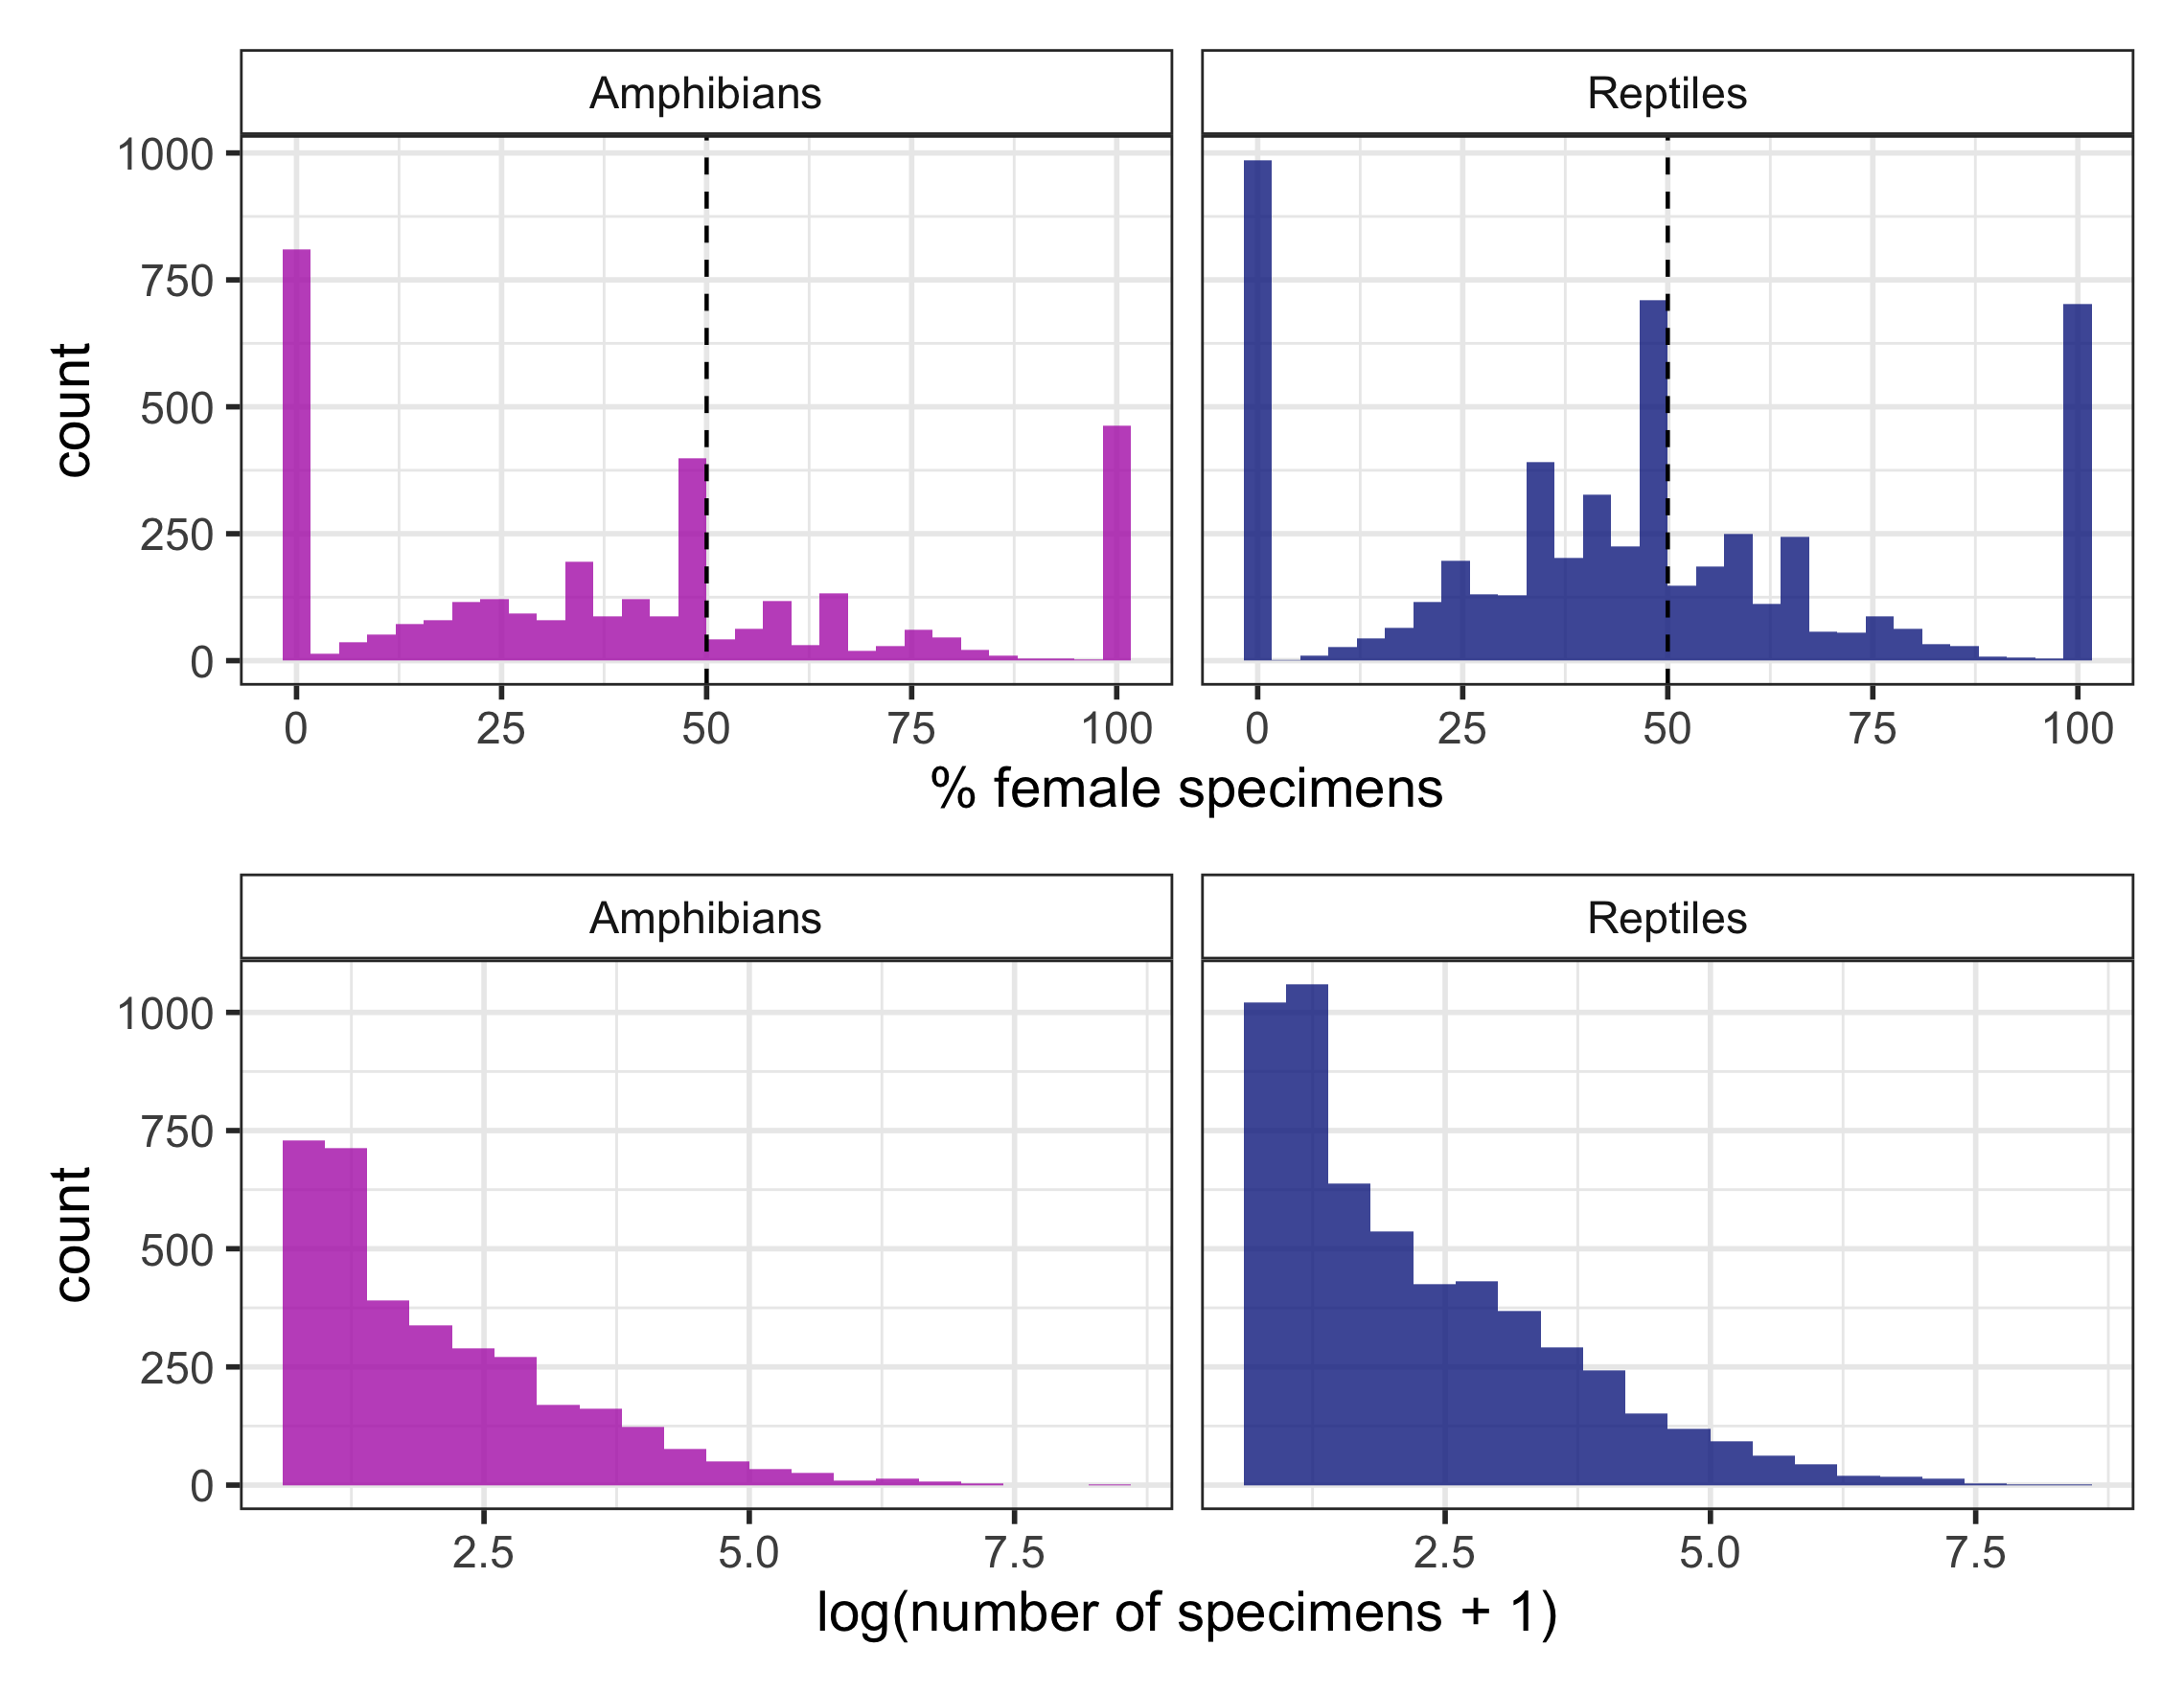
\includegraphics[width = \linewidth]{figures/histogram-specimen-counts.png}
  \caption{Histograms showing the distribution of percentage female specimens and log number of specimens for each species across amphibians and reptiles.}
  \label{fig-histograms}
\end{figure}

% figure A2
\begin{figure}[H]
 \centering
  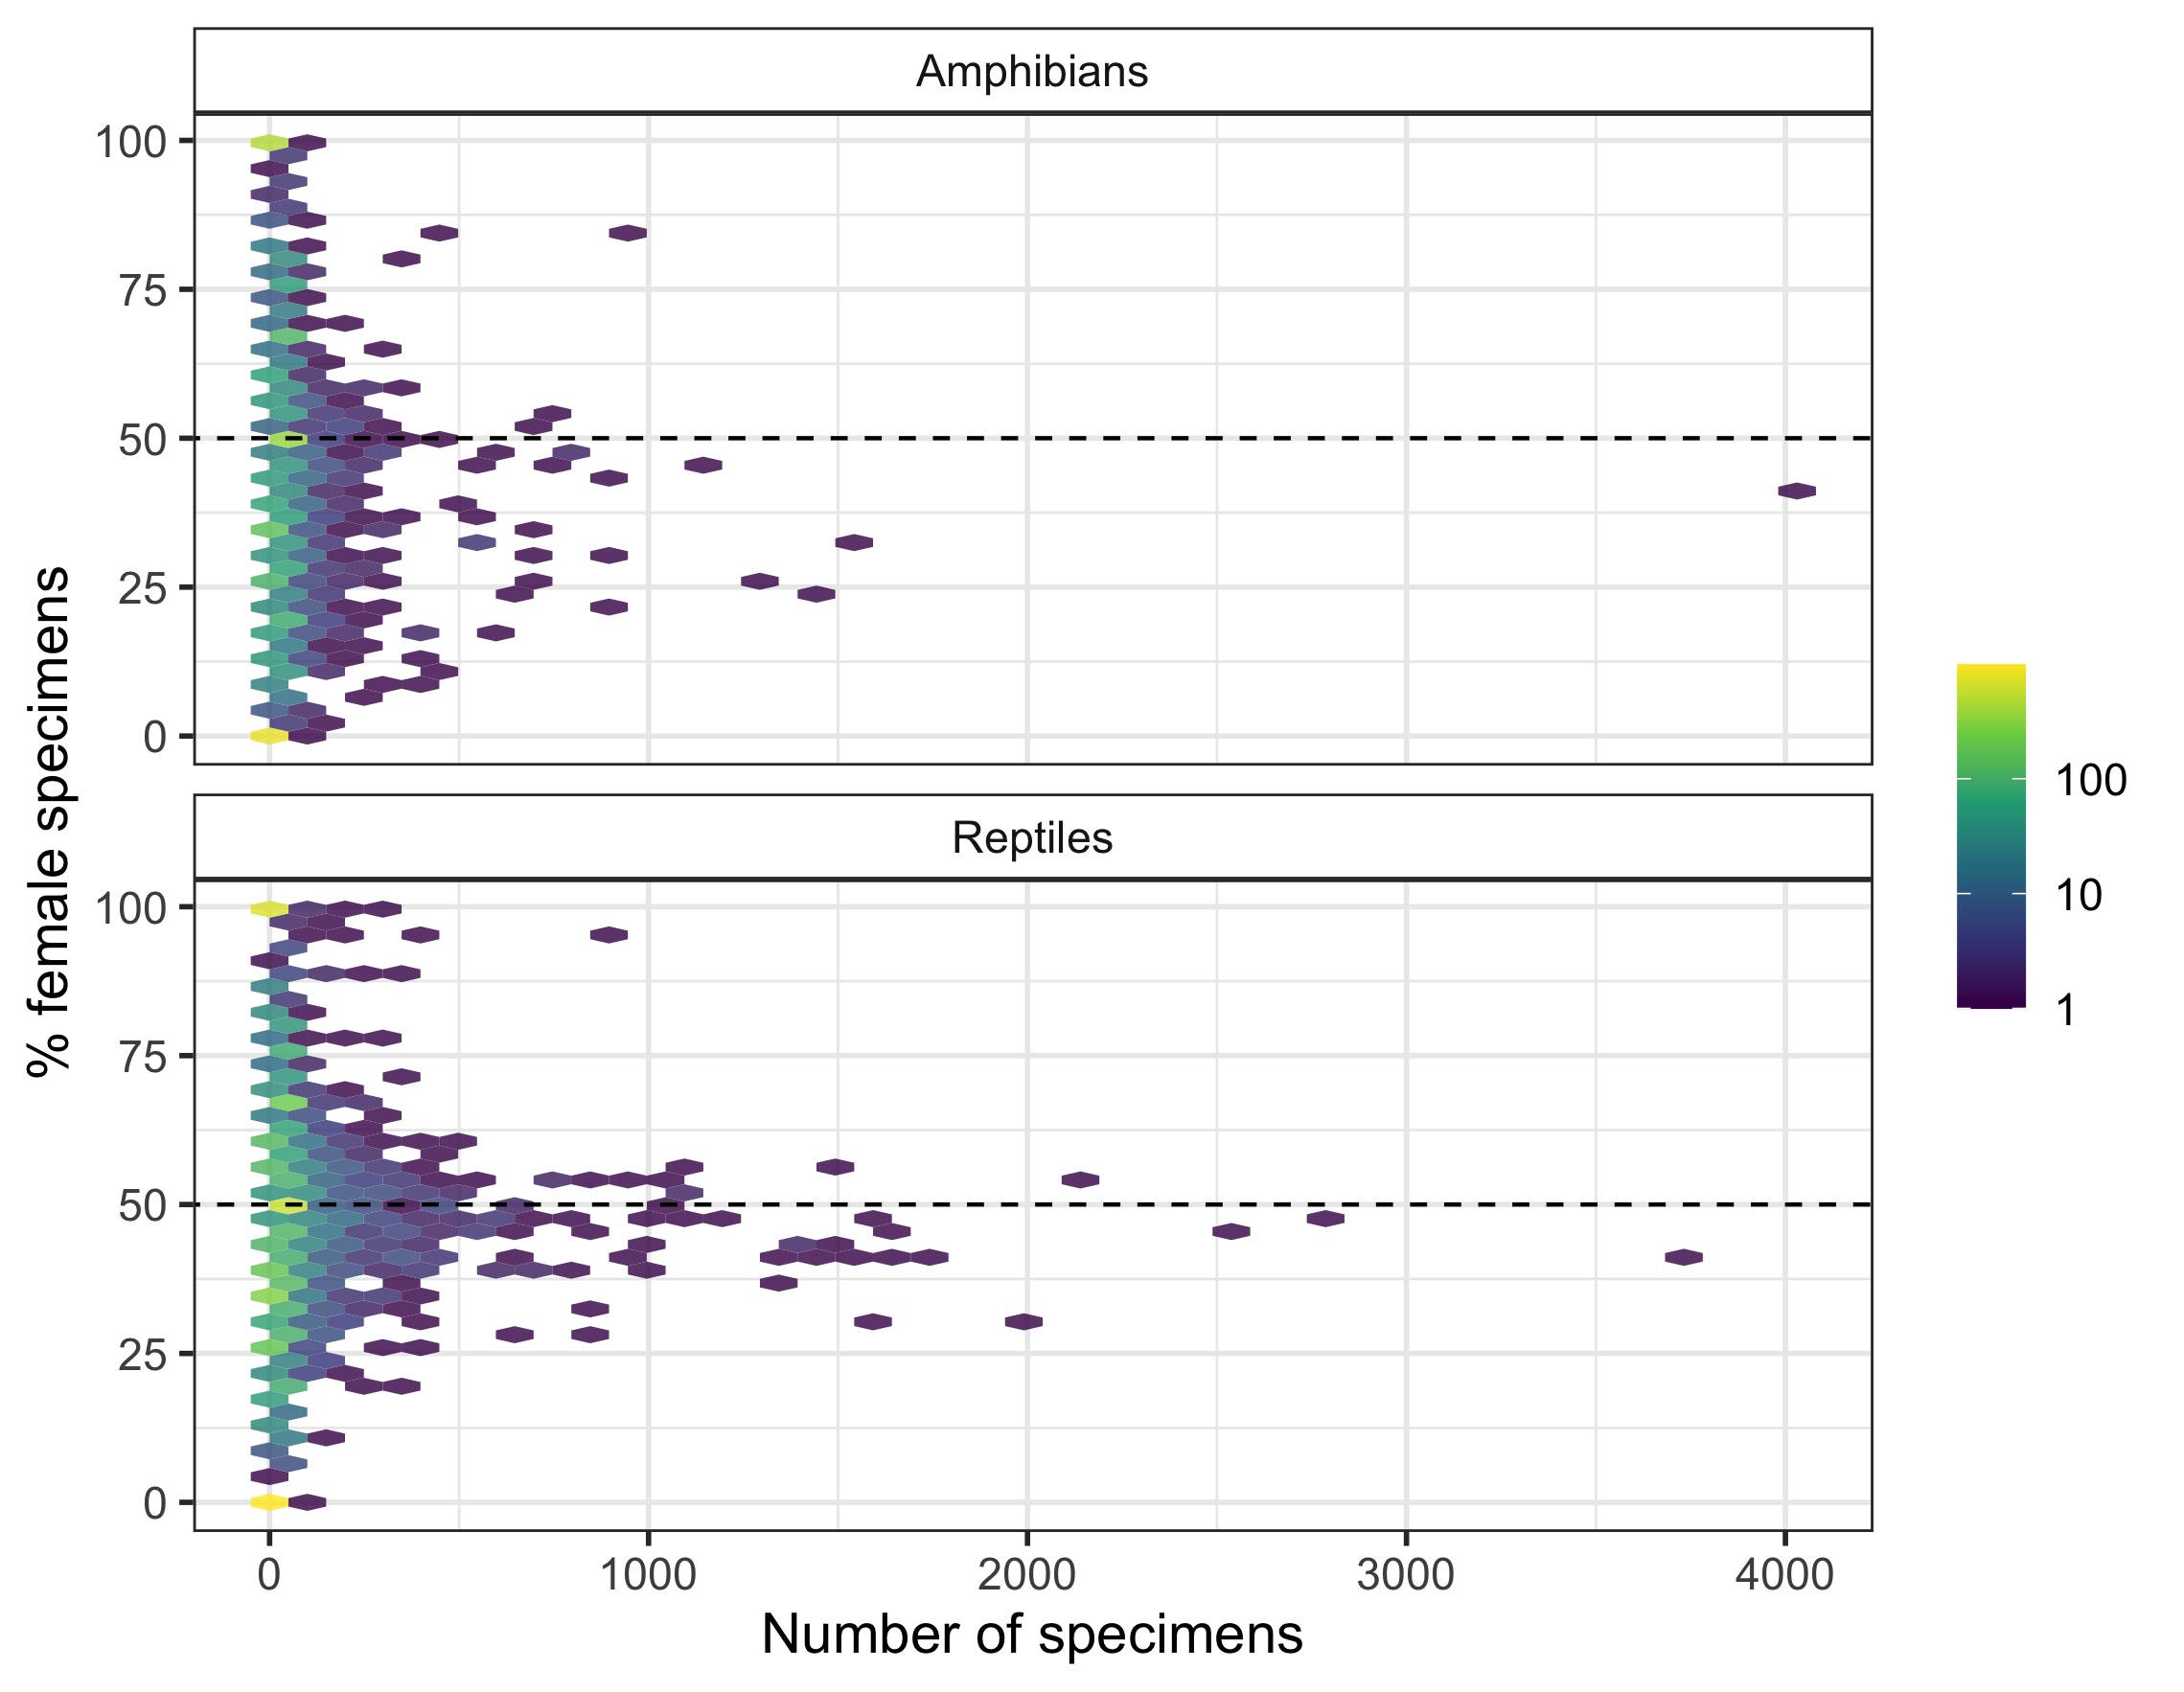
\includegraphics[width = \linewidth]{figures/specimens-numbers-all.png}
  \caption{Relationship between the percentage female specimens in each species and the number of specimens for each species across amphibians and reptiles. 
  Hex bins are used rather than points to make the plot easier to read.}
  \label{fig-hex}
\end{figure}

%-------------------------------------------------------------------------------
%\newpage
%\section{Genus-level data}

% Table A1
% \input{figures/table-genus}

%-------------------------------------------------------------------------------
\newpage
\section{Numbers of species and specimens in each analysis}

\begin{table}[H]
\centering
\begin{tabular}{cccc}

  \hline
  \textbf{Model} & \textbf{Specimens} & \textbf{median \% female} & \textbf{Species}\\ 
  \hline
  \textbf{Amphibians} & & &\\
  \hline
  orders & x & x & x\\
  years & x & x & x\\
  mass/SSD & x & x & x\\
  \hline
  \textbf{Reptiles} &&&\\
  \hline
  orders & x & x & x\\
  years & x & x & x\\
  mass/SSD & x & x & x\\
  \hline

\label{table_numbers}
\end{tabular}
\caption{Numbers of specimens and species in each of our models. SSD is sexual size dimorphism. All species have order data.} 

\end{table}
%-------------------------------------------------------------------------------
\newpage
\section{Total numbers of female specimens and female type specimens}

% figure A3
\begin{figure}[H]
 \centering
  \includegraphics[width = \linewidth]{figures/types-all.png}
  \caption{Percentages of female (green) and male (blue) specimens in bird and mammal collections for all specimens (left hand panel) and for name-bearing type specimens only (right hand panel). 
  The dashed line represents 50\% female specimens.}
  \label{fig-types}
\end{figure}

%-------------------------------------------------------------------------------
\newpage
\section{Exploring the unsexed specimen data}

49\% of bird specimens and 15\% of mammal specimens had no data on their sex at all. This is likely related to a number of factors. 
First, sexing birds and mammals is not always straightforward. Some species do not have clear external diagnostic features, so require dissection or close inspection by experts. 
In some bird species, for example, juvenile males and adult females may have very similar plumage, making differentiation difficult. 
Not all collectors or curators will have the skills to make these decisions, so collections remain unsexed. 
Second, historical collections often have poor metadata, in part because no-one imagined a time when you might examine the records without the specimen in front of you - as such many obviously male and female specimens are not recorded as such in specimen catalogues (this is common in the NHM collections \textit{pers. comm}).
 Curators and collections managers are often too busy to add these data when collections are massive and in need of much care and attention. 

We cannot sex all of the 687,393 unsexed bird and 161,526 unsexed mammals specimens in this study, instead we investigated variation in the numbers of unsexed specimens by order, collection continent and collection decade. 
Note that the figures below use all unsexed specimens, i.e. we did not exclude species with fewer than 100 specimens.

% figure A4
\begin{figure}[H]
 \centering
  \includegraphics[width = \linewidth]{figures/nosex-orders.png}
  \caption{Unsexed specimens across orders of birds and mammals. 
  Points are the mean percentage of unsexed specimens across all species within an order. 
  Error bars are standard errors.}
  \label{fig-nosex-orders}
\end{figure}

% figure A5
\begin{figure}[H]
 \centering
  \includegraphics[width = \linewidth]{figures/nosex-through-time.png}
  \caption{Unsexed specimens of birds and mammals across decades. 
  Lines show the mean percentage of unsexed specimens across all specimens collected within a given decade with 95\% confidence intervals.}
  \label{fig-nosex-decade}
\end{figure}

% figure A6
\begin{figure}[H]
 \centering
  \includegraphics[width = \linewidth]{figures/nosex-regions.png}
  \caption{Unsexed specimens of birds and mammals across continents they were collected in. 
  Points are the mean percentage of unsexed specimens across all species collected within a continent. 
  Error bars are standard errors.}
  \label{fig-nosex-continent}
\end{figure}

There is a lot of variation in the percentage of unsexed specimens across orders (Figure \ref{fig-nosex-orders}), regions (Figure \ref{fig-nosex-continent}) and through time (Figure \ref{fig-nosex-decade}). 
Interestingly, while the percentage of unsexed mammals has steadily decreased through time, in birds there is a steady decrease until 1900 followed by a slow increase towards the present. 
Patterns across orders and regions are not easily explained by the presence of hard to sex species.

\subsection*{Do unsexed specimens bias our results towards males?}

The presence of unsexed specimens may bias our results in various ways, but the worst possible scenario is that the majority of unsexed specimens are females, leading to the male bias we report in the main text. 
If this were true, we would expect the percentage of unsexed specimens to be strongly negatively correlated with the percentage of female specimens when we only consider female and male specimens. 
So, for example, a species with 50\% female and 50\% male specimens would have a higher percentage of unsexed specimens than one with 90\% female and 10\% male. 

We tested this by fitting linear models to compare the percentage of unsexed specimens (in species with more than 100 specimens overall) and the percentage of female specimens (in species with more than 100 sexed specimens). 
We investigated the correlation at two taxonomic levels 1) mean percentages within each order and 2) mean percentages within each species.

\subsubsection*{Within orders}
There were no significant correlations between the percentage of unsexed specimens and the percentage of female specimens across orders in either birds (linear regression: $slope ± SE = 0.143 \pm 0.359$, $t = 0.398$, $df = 23$, $p = 0.694$; Figure \ref{fig-nosex-correlation}) or mammals (linear regression: $slope \pm SE = 0.225 \pm 0.513$, $t = 0.439$, $df = 23$, $p = 0.665$; Figure \ref{fig-nosex-correlation}). 

% figure A7
\begin{figure}[H]
 \centering
  \includegraphics[width = \linewidth]{figures/nosex-correlation.png}
  \caption{The relationship between the percentage of female specimens and percentage of unsexed specimens across orders of birds and mammals. 
  Lines are from a linear regression, and shaded bars represent 95\% confidence intervals on the model.}
  \label{fig-nosex-correlation}
\end{figure}

\subsubsection*{Within species}
There was no significant correlation between the percentage of unsexed specimens and the percentage of female specimens across species in birds (linear regression: $slope \pm SE = 0.092 \pm 0.050$, $t = 1.876$, $df = 1743$, $p = 0.061$; Figure \ref{fig-nosex-correlation2}), but there was a weak negative correlation in mammals (linear regression: $slope \pm SE = -0.120 \pm 0.042$, $t = -2.852$, $df = 1487$, $p = 0.004$; Figure \ref{fig-nosex-correlation2}). 
The effect size was very small, however, so we do not place much emphasis on this result.

Note that without sexing the unsexed specimens we cannot be sure a bias does not exist, but the lack of correlation (except the weak one within species for mammals) makes us believe our results are likely not driven by unsexed specimens being predominantly female.

% figure A8
\begin{figure}[H]
 \centering
  \includegraphics[width = \linewidth]{figures/nosex-binomial-correlation.png}
  \caption{The relationship between the percentage of female specimens and percentage of unsexed specimens across species of birds and mammals.
  Lines are from a linear regression, and shaded bars represent 95\% confidence intervals on the model.}
  \label{fig-nosex-correlation2}
\end{figure}

%-------------------------------------------------------------------------------
\newpage
\section{Comparing our sex ratios to wild adult sex ratio data for birds}

There is very little available data on sex ratios in wild bird populations. The study which has collated the most data so far is Szekely et al. (2014). We took their data and compared the wild adult sex ratios (number of males/ number of males + number of females) to the sex ratios of the matching species in our dataset.

Overall we found 119 overlapping species out of the 187 in Szekely et al. (2014)\cite{szekely2014sex}.
Of these 88 (74\%) have less male biased sex ratios in the wild compared to museums, while the remaining 31 (26\%) have more male biased sex ratios in the wild compared to museums. 
This difference was significant (paired t-test: $t_{118} = -6.768$, $p < 0.001$; Figure \ref{fig-asr})

% figure A7
\begin{figure}[H]
 \centering
  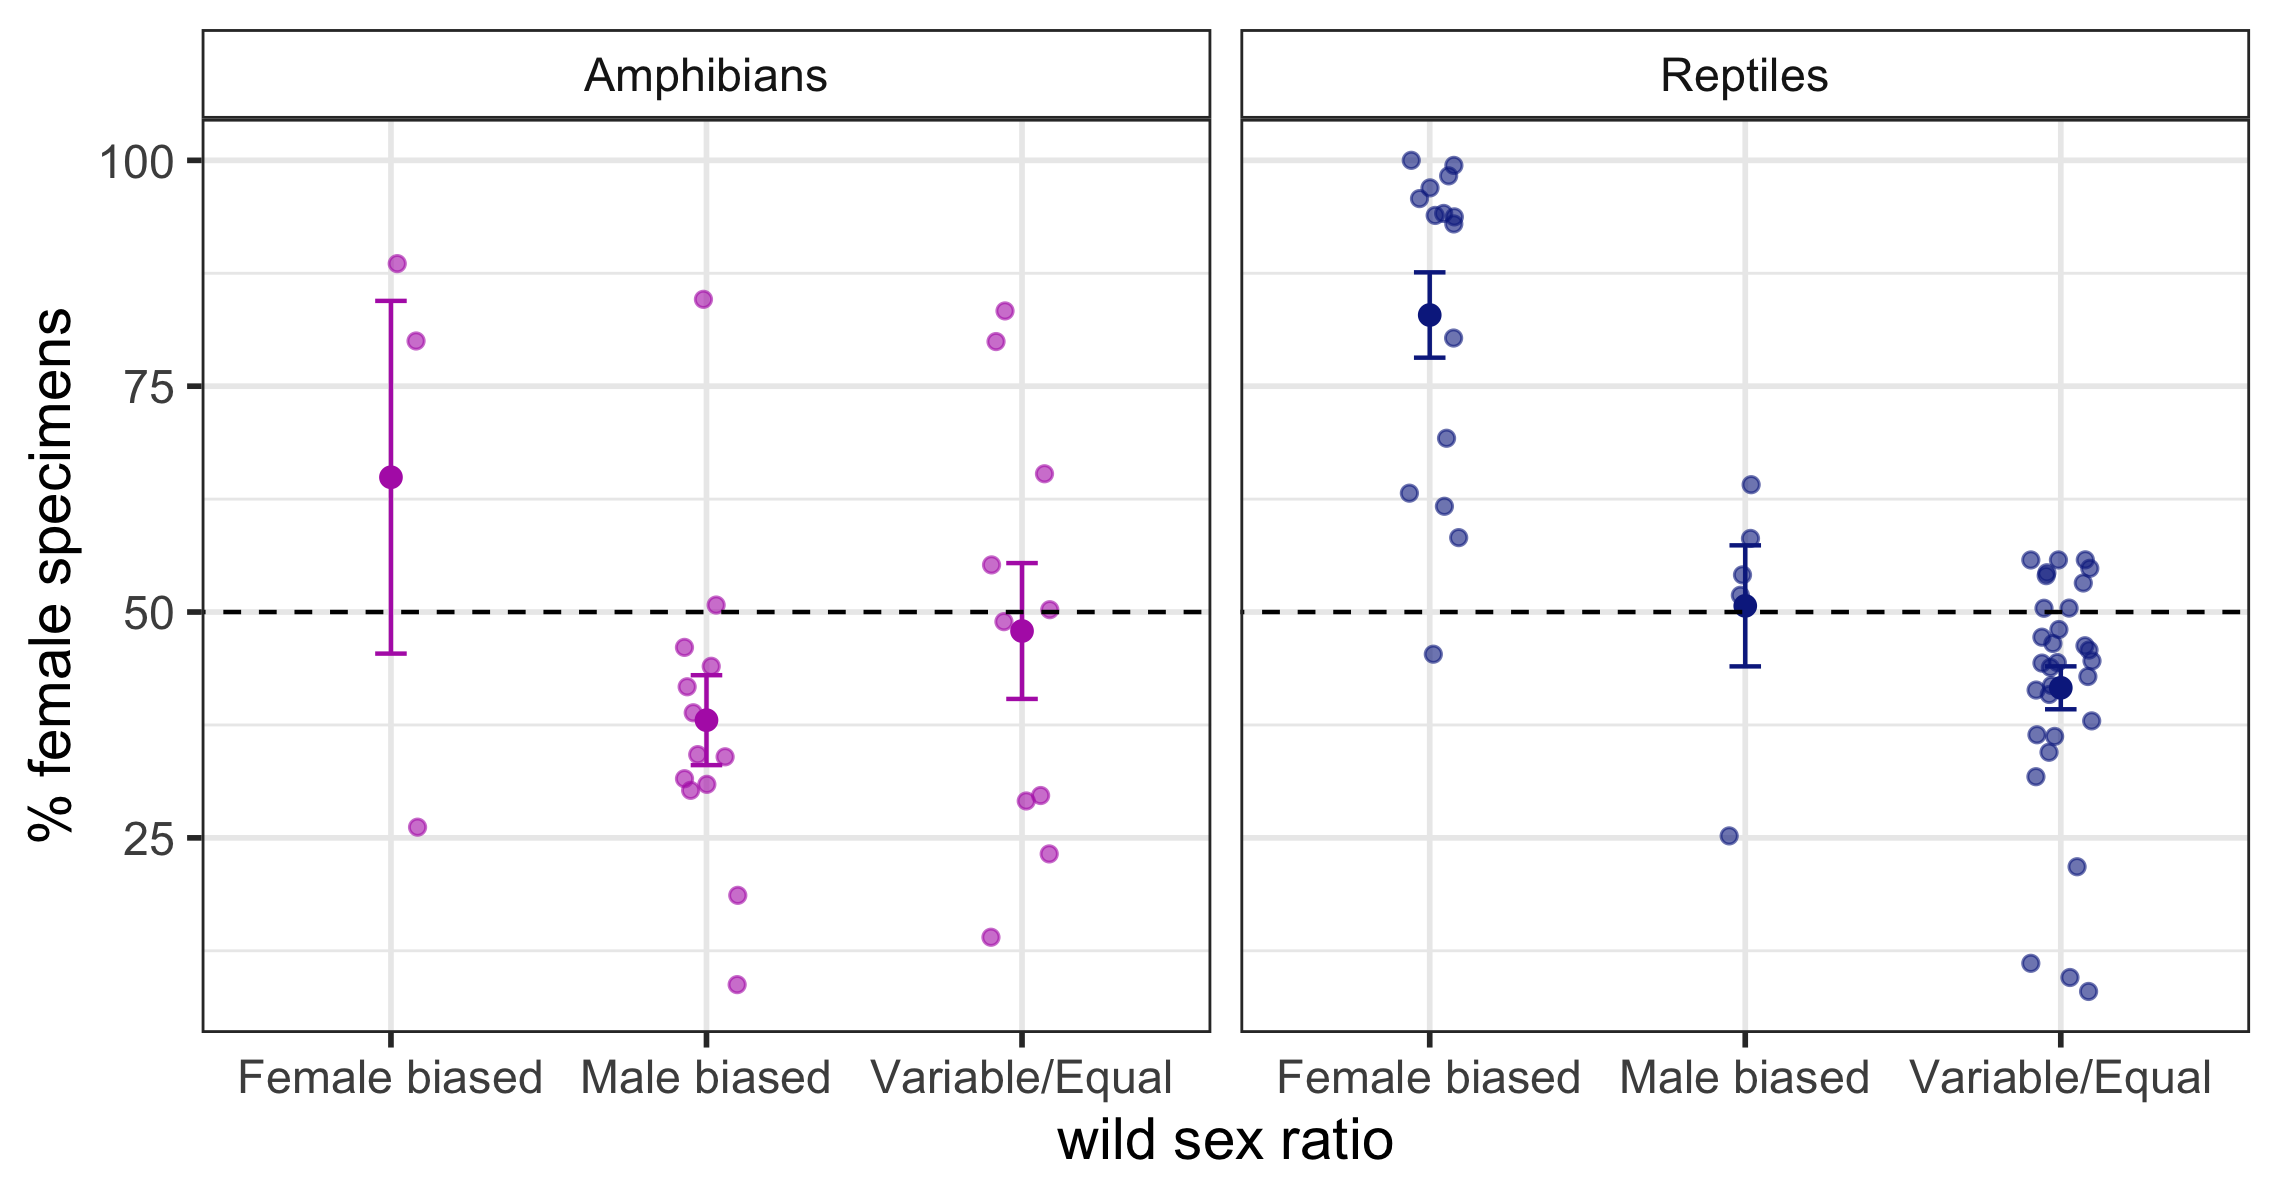
\includegraphics[width = \linewidth]{figures/wild-sex-ratios.png}
  \caption{Adult sex ratio (ASR) in wild populations versus ASR in our museum dataset for 119 bird species. 
  Wild ASR values come from Szekely et al. (2014)\cite{szekely2014sex}. 
  For the museum dataset only species with at least 100 specimens are included. 
  The dotted lines represents 50\% female specimens in either the wild or museum ASR data. 
  The red dashed line is the 1:1 line representing where points would sit of wild ASR and museum ASR are identical for a given species.
  Points above this line indicate species where museum ASR is more male biased than in wild populations.
}
  \label{fig-asr}
\end{figure}

%-------------------------------------------------------------------------------
\newpage
\section{Species with the most extreme sex ratios}
% Table A3
% latex table generated in R 4.1.0 by xtable 1.8-4 package
% Fri Aug  6 13:08:12 2021
\begin{longtable}{ll>{\itshape}lcc}
\caption{Species of amphibians and reptiles with the most extreme sex ratios
                  in our data, i.e. species with fewer than 25% female or fewer 
                  than 25% male specimens, for species with at least 10 specimens
                  in total. Species with  fewer than 25% male specimens are highlighted 
                  in bold.} \\ 
  \hline
class & order & binomial & n specimens & \% female \\ 
  \hline
Amphibians & Anura & Dendropsophus gaucheri & 121 & 1.65 \\ 
  Amphibians & Anura & Scinax alter &  51 & 1.96 \\ 
  Amphibians & Anura & Scinax boesemani &  74 & 2.70 \\ 
  Amphibians & Anura & Eleutherodactylus nitidus &  35 & 2.86 \\ 
  Amphibians & Anura & Boana polytaenia &  30 & 3.33 \\ 
  Amphibians & Anura & Aplastodiscus albosignatus &  28 & 3.57 \\ 
  Amphibians & Anura & Physalaemus ephippifer &  82 & 3.66 \\ 
  Amphibians & Anura & Breviceps gibbosus &  27 & 3.70 \\ 
  Amphibians & Anura & Boana multifasciata &  25 & 4.00 \\ 
  Amphibians & Anura & Phlyctimantis leonardi &  22 & 4.55 \\ 
  Amphibians & Anura & Phyllomedusa azurea &  21 & 4.76 \\ 
  Amphibians & Anura & Dendropsophus elegans &  61 & 4.92 \\ 
  Amphibians & Anura & Rhinella jimi &  40 & 5.00 \\ 
  Amphibians & Anura & Scinax squalirostris &  20 & 5.00 \\ 
  Amphibians & Anura & Oreolalax omeimontis &  18 & 5.56 \\ 
  Amphibians & Anura & Hyperolius baumanni &  18 & 5.56 \\ 
  Amphibians & Anura & Quasipaa spinosa &  18 & 5.56 \\ 
  Amphibians & Anura & Dendropsophus berthalutzae &  17 & 5.88 \\ 
  Amphibians & Anura & Pristimantis elegans &  32 & 6.25 \\ 
  Amphibians & Anura & Scinax exiguus &  16 & 6.25 \\ 
  Amphibians & Anura & Dendropsophus oliveirai &  16 & 6.25 \\ 
  Amphibians & Caudata & Euproctus montanus &  46 & 6.52 \\ 
  Amphibians & Anura & Leptobrachella oshanensis &  15 & 6.67 \\ 
  Amphibians & Anura & Leptobrachium mouhoti &  15 & 6.67 \\ 
  Amphibians & Anura & Ophryophryne hansi &  15 & 6.67 \\ 
  Amphibians & Anura & Boana semiguttata &  15 & 6.67 \\ 
  Amphibians & Anura & Boana heilprini &  15 & 6.67 \\ 
  Amphibians & Anura & Cophixalus sphagnicola &  14 & 7.14 \\ 
  Amphibians & Anura & Hyperolius nitidulus &  54 & 7.41 \\ 
  Amphibians & Anura & Scinax fuscomarginatus &  66 & 7.58 \\ 
  Amphibians & Anura & Dendropsophus nanus & 261 & 7.66 \\ 
  Amphibians & Anura & Dendropsophus minutus & 417 & 7.67 \\ 
  Amphibians & Anura & Amolops compotrix &  13 & 7.69 \\ 
  Amphibians & Anura & Pseudopaludicola ibisoroca &  13 & 7.69 \\ 
  Amphibians & Anura & Scinax perereca &  13 & 7.69 \\ 
  Amphibians & Anura & Eleutherodactylus wightmanae &  13 & 7.69 \\ 
  Amphibians & Caudata & Hynobius retardatus &  26 & 7.69 \\ 
  Amphibians & Anura & Microhyla okinavensis &  26 & 7.69 \\ 
  Amphibians & Anura & Pleurodema tucumanum &  13 & 7.69 \\ 
  Amphibians & Anura & Eleutherodactylus pentasyringos &  26 & 7.69 \\ 
  Amphibians & Anura & Glyphoglossus yunnanensis &  12 & 8.33 \\ 
  Amphibians & Anura & Hyla annectans &  12 & 8.33 \\ 
  Amphibians & Anura & Eleutherodactylus rhodesi &  12 & 8.33 \\ 
  Amphibians & Anura & Rhacophorus margaritifer &  12 & 8.33 \\ 
  Amphibians & Anura & Platymantis mimulus &  12 & 8.33 \\ 
  Amphibians & Anura & Platymantis polillensis &  12 & 8.33 \\ 
  Amphibians & Anura & Sclerophrys steindachneri &  12 & 8.33 \\ 
  Amphibians & Anura & Rhinella ornata &  12 & 8.33 \\ 
  Amphibians & Anura & Hyloscirtus phyllognathus &  12 & 8.33 \\ 
  Amphibians & Anura & Boana callipleura &  12 & 8.33 \\ 
  Amphibians & Anura & Peltophryne guentheri &  23 & 8.70 \\ 
  Amphibians & Anura & Afrixalus delicatus &  11 & 9.09 \\ 
  Amphibians & Anura & Huia cavitympanum &  33 & 9.09 \\ 
  Amphibians & Anura & Eleutherodactylus auriculatus &  11 & 9.09 \\ 
  Amphibians & Anura & Phyllomedusa nordestina &  11 & 9.09 \\ 
  Amphibians & Anura & Litoria freycineti &  11 & 9.09 \\ 
  Amphibians & Anura & Hyla andersonii & 277 & 9.39 \\ 
  Amphibians & Anura & Boana sibleszi &  42 & 9.52 \\ 
  Amphibians & Anura & Leptodactylus notoaktites &  21 & 9.52 \\ 
  Amphibians & Anura & Litoria nigropunctata &  21 & 9.52 \\ 
  Amphibians & Anura & Dendropsophus bipunctatus & 142 & 9.86 \\ 
  Amphibians & Anura & Rhacophorus bipunctatus &  10 & 10.00 \\ 
  Amphibians & Anura & Xenophrys periosa &  10 & 10.00 \\ 
  Amphibians & Anura & Boana riojana &  20 & 10.00 \\ 
  Amphibians & Anura & Litoria prora &  10 & 10.00 \\ 
  Amphibians & Anura & Leptophryne borbonica &  10 & 10.00 \\ 
  Amphibians & Anura & Strongylopus grayii &  10 & 10.00 \\ 
  Amphibians & Anura & Mantidactylus femoralis &  10 & 10.00 \\ 
  Amphibians & Anura & Teratohyla spinosa &  10 & 10.00 \\ 
  Amphibians & Anura & Eleutherodactylus cavernicola &  10 & 10.00 \\ 
  Amphibians & Anura & Hyperolius endjami &  20 & 10.00 \\ 
  Amphibians & Anura & Hyperolius lateralis &  29 & 10.34 \\ 
  Amphibians & Anura & Crossodactylus caramaschii &  67 & 10.45 \\ 
  Amphibians & Anura & Boana albomarginata & 430 & 10.47 \\ 
  Amphibians & Anura & Eleutherodactylus auriculatoides &  19 & 10.53 \\ 
  Amphibians & Anura & Hyalinobatrachium valerioi &  19 & 10.53 \\ 
  Amphibians & Anura & Pseudacris kalmi &  19 & 10.53 \\ 
  Amphibians & Anura & Hyperolius drewesi &  66 & 10.61 \\ 
  Amphibians & Anura & Amolops archotaphus &  28 & 10.71 \\ 
  Amphibians & Anura & Heleioporus albopunctatus &  18 & 11.11 \\ 
  Amphibians & Anura & Eleutherodactylus andrewsi &  27 & 11.11 \\ 
  Amphibians & Anura & Nyctimystes cheesmani &  27 & 11.11 \\ 
  Amphibians & Anura & Atelopus chiriquiensis &  35 & 11.43 \\ 
  Amphibians & Anura & Alytes obstetricans &  43 & 11.63 \\ 
  Amphibians & Anura & Hyperolius camerunensis &  34 & 11.76 \\ 
  Amphibians & Anura & Dendropsophus microcephalus & 136 & 11.76 \\ 
  Amphibians & Anura & Brachytarsophrys intermedia &  17 & 11.76 \\ 
  Amphibians & Anura & Pristimantis reichlei &  17 & 11.76 \\ 
  Amphibians & Anura & Bufotes latastii &  41 & 12.20 \\ 
  Amphibians & Anura & Atelopus spumarius &  49 & 12.24 \\ 
  Amphibians & Anura & Kassina cassinoides &  16 & 12.50 \\ 
  Amphibians & Anura & Phyllomedusa vaillantii &  16 & 12.50 \\ 
  Amphibians & Anura & Hyperolius quinquevittatus &  16 & 12.50 \\ 
  Amphibians & Anura & Rana pirica &  16 & 12.50 \\ 
  Amphibians & Anura & Phyllomedusa camba &  16 & 12.50 \\ 
  Amphibians & Anura & Pseudacris streckeri &  87 & 12.64 \\ 
  Amphibians & Anura & Dendropsophus sanborni &  38 & 13.16 \\ 
  Amphibians & Anura & Boana albopunctata & 120 & 13.33 \\ 
  Amphibians & Anura & Eleutherodactylus locustus &  15 & 13.33 \\ 
  Amphibians & Anura & Osteocephalus verruciger &  15 & 13.33 \\ 
  Amphibians & Anura & Aplastodiscus perviridis &  15 & 13.33 \\ 
  Amphibians & Anura & Platymantis browni &  30 & 13.33 \\ 
  Amphibians & Anura & Hyperolius riggenbachi &  67 & 13.43 \\ 
  Amphibians & Anura & Scinax x-signatus &  52 & 13.46 \\ 
  Amphibians & Anura & Scinax fuscovarius &  37 & 13.51 \\ 
  Amphibians & Anura & Eleutherodactylus schmidti &  37 & 13.51 \\ 
  Amphibians & Anura & Hyla versicolor & 440 & 13.64 \\ 
  Amphibians & Anura & Scutiger sikimmensis &  88 & 13.64 \\ 
  Amphibians & Anura & Exerodonta xera &  22 & 13.64 \\ 
  Amphibians & Anura & Chalcorana chalconota & 219 & 13.70 \\ 
  Amphibians & Anura & Physalaemus cuvieri & 247 & 13.77 \\ 
  Amphibians & Anura & Boana lanciformis &  29 & 13.79 \\ 
  Amphibians & Anura & Anaxyrus baxteri &  36 & 13.89 \\ 
  Amphibians & Caudata & Tylototriton uyenoi &  36 & 13.89 \\ 
  Amphibians & Anura & Eleutherodactylus brevirostris &  14 & 14.29 \\ 
  Amphibians & Anura & Eleutherodactylus weinlandi &  14 & 14.29 \\ 
  Amphibians & Anura & Eleutherodactylus haitianus &  14 & 14.29 \\ 
  Amphibians & Anura & Phyllomedusa tomopterna &  28 & 14.29 \\ 
  Amphibians & Anura & Hyla wrightorum &  21 & 14.29 \\ 
  Amphibians & Anura & Pseudis bolbodactyla &  14 & 14.29 \\ 
  Amphibians & Anura & Micryletta inornata & 109 & 14.68 \\ 
  Amphibians & Anura & Buergeria buergeri &  81 & 14.81 \\ 
  Amphibians & Anura & Dendropsophus bifurcus &  20 & 15.00 \\ 
  Amphibians & Anura & Centrolene hesperium &  20 & 15.00 \\ 
  Amphibians & Anura & Dendropsophus sarayacuensis &  39 & 15.38 \\ 
  Amphibians & Anura & Myersiohyla neblinaria &  13 & 15.38 \\ 
  Amphibians & Anura & Crossodactylus aeneus &  13 & 15.38 \\ 
  Amphibians & Anura & Dendropsophus acreanus &  13 & 15.38 \\ 
  Amphibians & Anura & Anomaloglossus baeobatrachus &  26 & 15.38 \\ 
  Amphibians & Anura & Hyperolius balfouri &  19 & 15.79 \\ 
  Amphibians & Anura & Physalaemus albonotatus &  19 & 15.79 \\ 
  Amphibians & Anura & Vandijkophrynus amatolicus &  19 & 15.79 \\ 
  Amphibians & Anura & Panophrys omeimontis &  19 & 15.79 \\ 
  Amphibians & Anura & Xenopus muelleri &  57 & 15.79 \\ 
  Amphibians & Anura & Agalychnis dacnicolor &  31 & 16.13 \\ 
  Amphibians & Anura & Hyla chrysoscelis & 566 & 16.61 \\ 
  Amphibians & Anura & Pithecopus hypochondrialis &  84 & 16.67 \\ 
  Amphibians & Anura & Eleutherodactylus alticola &  18 & 16.67 \\ 
  Amphibians & Anura & Osteopilus pulchrilineatus &  36 & 16.67 \\ 
  Amphibians & Anura & Chiromantis doriae &  18 & 16.67 \\ 
  Amphibians & Anura & Rana chaochiaoensis &  12 & 16.67 \\ 
  Amphibians & Anura & Phyllomedusa tetraploidea &  18 & 16.67 \\ 
  Amphibians & Anura & Boana semilineata &  12 & 16.67 \\ 
  Amphibians & Anura & Xenopus longipes &  12 & 16.67 \\ 
  Amphibians & Anura & Phrynobatrachus gutturosus &  35 & 17.14 \\ 
  Amphibians & Anura & Tlalocohyla loquax &  29 & 17.24 \\ 
  Amphibians & Caudata & Desmognathus aeneus &  29 & 17.24 \\ 
  Amphibians & Anura & Eleutherodactylus portoricensis &  23 & 17.39 \\ 
  Amphibians & Anura & Eleutherodactylus patriciae &  23 & 17.39 \\ 
  Amphibians & Anura & Tepuihyla obscura &  46 & 17.39 \\ 
  Amphibians & Anura & Leptopelis ocellatus &  34 & 17.65 \\ 
  Amphibians & Anura & Meristogenys phaeomerus &  34 & 17.65 \\ 
  Amphibians & Anura & Sphaenorhynchus caramaschii &  17 & 17.65 \\ 
  Amphibians & Anura & Eleutherodactylus cochranae &  17 & 17.65 \\ 
  Amphibians & Anura & Pseudacris nigrita & 435 & 17.70 \\ 
  Amphibians & Anura & Bombina bombina &  56 & 17.86 \\ 
  Amphibians & Anura & Hyperolius ocellatus &  89 & 17.98 \\ 
  Amphibians & Anura & Ingerophrynus celebensis & 371 & 18.06 \\ 
  Amphibians & Anura & Boana calcarata &  22 & 18.18 \\ 
  Amphibians & Anura & Hyperolius kivuensis &  22 & 18.18 \\ 
  Amphibians & Anura & Triprion petasatus &  11 & 18.18 \\ 
  Amphibians & Anura & Pseudacris clarkii &  22 & 18.18 \\ 
  Amphibians & Anura & Hyperolius spinigularis &  11 & 18.18 \\ 
  Amphibians & Anura & Limnonectes megastomias &  11 & 18.18 \\ 
  Amphibians & Anura & Dendropsophus decipiens &  11 & 18.18 \\ 
  Amphibians & Anura & Kaloula rigida &  11 & 18.18 \\ 
  Amphibians & Anura & Scutiger occidentalis &  66 & 18.18 \\ 
  Amphibians & Anura & Spea bombifrons & 115 & 18.26 \\ 
  Amphibians & Anura & Pulchrana signata & 120 & 18.33 \\ 
  Amphibians & Anura & Pseudacris brimleyi & 147 & 18.37 \\ 
  Amphibians & Anura & Ranoidea rheocola &  27 & 18.52 \\ 
  Amphibians & Anura & Odorrana hosii & 210 & 18.57 \\ 
  Amphibians & Anura & Acris gryllus & 199 & 18.59 \\ 
  Amphibians & Anura & Pseudacris brachyphona &  64 & 18.75 \\ 
  Amphibians & Anura & Semnodactylus wealii &  16 & 18.75 \\ 
  Amphibians & Anura & Kurixalus appendiculatus &  32 & 18.75 \\ 
  Amphibians & Anura & Phrynomantis microps &  16 & 18.75 \\ 
  Amphibians & Anura & Bokermannohyla hylax &  16 & 18.75 \\ 
  Amphibians & Anura & Rhinella magnussoni &  16 & 18.75 \\ 
  Amphibians & Anura & Amolops afghanus &  48 & 18.75 \\ 
  Amphibians & Anura & Pristimantis bogotensis &  53 & 18.87 \\ 
  Amphibians & Anura & Hyperolius puncticulatus & 153 & 18.95 \\ 
  Amphibians & Anura & Ranoidea nannotis &  21 & 19.05 \\ 
  Amphibians & Anura & Zhangixalus omeimontis &  21 & 19.05 \\ 
  Amphibians & Anura & Dendropsophus counani &  21 & 19.05 \\ 
  Amphibians & Anura & Smilisca fodiens &  26 & 19.23 \\ 
  Amphibians & Anura & Dendropsophus microps &  26 & 19.23 \\ 
  Amphibians & Anura & Pelobates syriacus &  26 & 19.23 \\ 
  Amphibians & Anura & Diasporus diastema &  56 & 19.64 \\ 
  Amphibians & Anura & Pseudopaludicola mystacalis & 112 & 19.64 \\ 
  Amphibians & Anura & Dendropsophus leucophyllatus &  61 & 19.67 \\ 
  Amphibians & Caudata & Ambystoma macrodactylum & 121 & 19.83 \\ 
  Amphibians & Anura & Pseudophilautus leucorhinus &  10 & 20.00 \\ 
  Amphibians & Anura & Sclerophrys langanoensis &  10 & 20.00 \\ 
  Amphibians & Caudata & Lissotriton graecus &  10 & 20.00 \\ 
  Amphibians & Anura & Indosylvirana indica &  10 & 20.00 \\ 
  Amphibians & Anura & Raorchestes chromasynchysi &  10 & 20.00 \\ 
  Amphibians & Anura & Leptodactylus bufonius &  50 & 20.00 \\ 
  Amphibians & Anura & Afrixalus vittiger &  15 & 20.00 \\ 
  Amphibians & Anura & Sclerophrys pentoni &  15 & 20.00 \\ 
  Amphibians & Anura & Hamptophryne boliviana &  10 & 20.00 \\ 
  Amphibians & Anura & Boana lemai &  15 & 20.00 \\ 
  Amphibians & Anura & Dendropsophus melanargyreus &  10 & 20.00 \\ 
  Amphibians & Anura & Pristimantis toftae &  10 & 20.00 \\ 
  Amphibians & Anura & Papurana celebensis &  79 & 20.25 \\ 
  Amphibians & Anura & Spea hammondii &  98 & 20.41 \\ 
  Amphibians & Anura & Rana arvalis &  44 & 20.45 \\ 
  Amphibians & Anura & Hyperolius molleri &  44 & 20.45 \\ 
  Amphibians & Anura & Eleutherodactylus pinchoni &  44 & 20.45 \\ 
  Amphibians & Anura & Rhacophorus edentulus &  44 & 20.45 \\ 
  Amphibians & Anura & Hyperolius olivaceus &  78 & 20.51 \\ 
  Amphibians & Anura & Eleutherodactylus glaphycompus &  34 & 20.59 \\ 
  Amphibians & Anura & Pseudacris triseriata & 257 & 20.62 \\ 
  Amphibians & Anura & Kassina arboricola &  29 & 20.69 \\ 
  Amphibians & Anura & Hyla avivoca &  48 & 20.83 \\ 
  Amphibians & Anura & Pseudis minuta &  24 & 20.83 \\ 
  Amphibians & Anura & Hyla japonica &  81 & 20.99 \\ 
  Amphibians & Anura & Pseudacris maculata & 257 & 21.01 \\ 
  Amphibians & Anura & Ranoidea eucnemis &  19 & 21.05 \\ 
  Amphibians & Anura & Pulchrana picturata &  19 & 21.05 \\ 
  Amphibians & Anura & Boana crepitans &  90 & 21.11 \\ 
  Amphibians & Anura & Hyperolius concolor & 210 & 21.43 \\ 
  Amphibians & Anura & Hyperolius mosaicus &  14 & 21.43 \\ 
  Amphibians & Anura & Leptopelis christyi &  14 & 21.43 \\ 
  Amphibians & Anura & Xenopus kobeli &  14 & 21.43 \\ 
  Amphibians & Anura & Hyla sarda &  14 & 21.43 \\ 
  Amphibians & Anura & Dendropsophus branneri &  51 & 21.57 \\ 
  Amphibians & Anura & Afrixalus nigeriensis &  23 & 21.74 \\ 
  Amphibians & Anura & Boana raniceps &  78 & 21.79 \\ 
  Amphibians & Anura & Hyla squirella & 876 & 21.80 \\ 
  Amphibians & Anura & Leptopelis aubryi &  73 & 21.92 \\ 
  Amphibians & Anura & Afrixalus paradorsalis &  36 & 22.22 \\ 
  Amphibians & Anura & Anaxyrus exsul &  22 & 22.73 \\ 
  Amphibians & Anura & Pseudopaludicola florencei &  22 & 22.73 \\ 
  Amphibians & Anura & Rheohyla miotympanum &  48 & 22.92 \\ 
  Amphibians & Anura & Hyperolius nasutus &  61 & 22.95 \\ 
  Amphibians & Anura & Hyperolius castaneus &  13 & 23.08 \\ 
  Amphibians & Anura & Phyllomedusa palliata &  13 & 23.08 \\ 
  Amphibians & Anura & Hyperolius mitchelli &  39 & 23.08 \\ 
  Amphibians & Anura & Cycloramphus boraceiensis &  13 & 23.08 \\ 
  Amphibians & Anura & Limnonectes microtympanum &  30 & 23.33 \\ 
  Amphibians & Anura & Proceratophrys boiei &  17 & 23.53 \\ 
  Amphibians & Anura & Leptopelis aubryioides &  17 & 23.53 \\ 
  Amphibians & Anura & Sanguirana luzonensis &  85 & 23.53 \\ 
  Amphibians & Anura & Leptodactylus rhodomystax &  17 & 23.53 \\ 
  Amphibians & Anura & Rana dalmatina & 136 & 23.53 \\ 
  Amphibians & Anura & Eleutherodactylus cundalli &  34 & 23.53 \\ 
  Amphibians & Anura & Eleutherodactylus riparius &  17 & 23.53 \\ 
  Amphibians & Caudata & Bolitoglossa carri &  17 & 23.53 \\ 
  Amphibians & Anura & Atelopus hoogmoedi &  34 & 23.53 \\ 
  Amphibians & Anura & Rana pyrenaica &  17 & 23.53 \\ 
  Amphibians & Anura & Kassina cochranae &  38 & 23.68 \\ 
  Amphibians & Anura & Pseudacris crucifer & 1464 & 23.84 \\ 
  Amphibians & Anura & Eleutherodactylus nubicola &  71 & 23.94 \\ 
  Amphibians & Anura & Boana faber & 125 & 24.00 \\ 
  Amphibians & Anura & Rana kauffeldi &  25 & 24.00 \\ 
  Amphibians & Anura & Rana graeca &  54 & 24.07 \\ 
  Amphibians & Anura & Boana pardalis &  87 & 24.14 \\ 
  Amphibians & Anura & Hyperolius cinnamomeoventris &  58 & 24.14 \\ 
  Amphibians & Anura & Pseudacris feriarum & 678 & 24.19 \\ 
  Amphibians & Anura & Hoplophryne uluguruensis &  33 & 24.24 \\ 
  Amphibians & Anura & Meristogenys poecilus & 123 & 24.39 \\ 
  Amphibians & Anura & Chiromantis xerampelina &  21 & 76.19 \\ 
  Amphibians & Anura & Vandijkophrynus angusticeps &  13 & 76.92 \\ 
  Amphibians & Anura & Leptopelis boulengeri &  13 & 76.92 \\ 
  Amphibians & Anura & Pseudophryne australis &  13 & 76.92 \\ 
  Amphibians & Caudata & Pseudotriton montanus &  13 & 76.92 \\ 
  Amphibians & Anura & Pristimantis bacchus &  13 & 76.92 \\ 
  Amphibians & Caudata & Pseudotriton ruber &  88 & 77.27 \\ 
  Amphibians & Anura & Phrynobatrachus alleni &  23 & 78.26 \\ 
  Amphibians & Caudata & Desmognathus ocoee &  81 & 79.01 \\ 
  Amphibians & Anura & Phrynobatrachus calcaratus &  29 & 79.31 \\ 
  Amphibians & Caudata & Ambystoma jeffersonianum & 311 & 79.42 \\ 
  Amphibians & Anura & Sclerophrys funerea &  10 & 80.00 \\ 
  Amphibians & Anura & Gephyromantis ambohitra &  15 & 80.00 \\ 
  Amphibians & Caudata & Desmognathus carolinensis &  26 & 80.77 \\ 
  Amphibians & Anura & Kalophrynus pleurostigma &  16 & 81.25 \\ 
  Amphibians & Anura & Eleutherodactylus pictissimus &  11 & 81.82 \\ 
  Amphibians & Caudata & Eurycea chamberlaini &  11 & 81.82 \\ 
  Amphibians & Anura & Hypopachus barberi &  11 & 81.82 \\ 
  Amphibians & Anura & Cophixalus verrucosus &  17 & 82.35 \\ 
  Amphibians & Anura & Austrochaperina palmipes &  58 & 82.76 \\ 
  Amphibians & Anura & Ingerophrynus biporcatus &  12 & 83.33 \\ 
  Amphibians & Anura & Astylosternus occidentalis &  18 & 83.33 \\ 
  Amphibians & Anura & Cornufer pelewensis & 400 & 84.25 \\ 
  Amphibians & Caudata & Plethodon cinereus & 926 & 84.99 \\ 
  Amphibians & Anura & Chiasmocleis schubarti &  30 & 86.67 \\ 
  Amphibians & Caudata & Hemidactylium scutatum &  62 & 87.10 \\ 
  Amphibians & Caudata & Plethodon hubrichti &  59 & 88.14 \\ 
  Amphibians & Anura & Craugastor fleischmanni &  17 & 88.24 \\ 
  Amphibians & Anura & Pristimantis chimu &  18 & 88.89 \\ 
  Amphibians & Anura & Eleutherodactylus furcyensis &  20 & 90.00 \\ 
  Amphibians & Anura & Hylorina sylvatica &  10 & 90.00 \\ 
  Amphibians & Anura & Pristimantis dundeei &  50 & 92.00 \\ 
  Amphibians & Anura & Hyperolius substriatus &  13 & 92.31 \\ 
  Amphibians & Caudata & Batrachoseps wrighti &  14 & 92.86 \\ 
  Amphibians & Anura & Pristimantis petrobardus &  18 & 94.44 \\ 
  Amphibians & Anura & Gastrotheca peruana &  33 & 96.97 \\ 
  Amphibians & Anura & Incilius ibarrai &  37 & 97.30 \\ 
  Amphibians & Anura & Nectophrynoides tornieri &  66 & 98.48 \\ 
  Amphibians & Caudata & Plethodon hoffmani &  53 & 100.00 \\ 
  Amphibians & Anura & Pristimantis cerasinus &  14 & 100.00 \\ 
  Amphibians & Anura & Aphantophryne sabini &  15 & 100.00 \\ 
  Amphibians & Anura & Staurois latopalmatus &  24 & 100.00 \\ 
  Amphibians & Anura & Staurois guttatus &  15 & 100.00 \\ 
  Amphibians & Anura & Meristogenys orphnocnemis &  13 & 100.00 \\ 
  Reptiles & Squamata & Emoia guttata & 103 & 0.97 \\ 
  Reptiles & Squamata & Trioceros fuelleborni &  21 & 4.76 \\ 
  Reptiles & Squamata & Emoia nigromarginata &  17 & 5.88 \\ 
  Reptiles & Squamata & Trachylepis albilabris &  17 & 5.88 \\ 
  Reptiles & Squamata & Calumma gallus &  15 & 6.67 \\ 
  Reptiles & Squamata & Emoia boettgeri &  29 & 6.90 \\ 
  Reptiles & Squamata & Scincella vandenburghi &  14 & 7.14 \\ 
  Reptiles & Squamata & Cophoscincopus simulans &  27 & 7.41 \\ 
  Reptiles & Squamata & Varanus gouldii &  12 & 8.33 \\ 
  Reptiles & Squamata & Cryptoblepharus eximius &  36 & 8.33 \\ 
  Reptiles & Squamata & Tantillita lintoni &  12 & 8.33 \\ 
  Reptiles & Squamata & Ahaetulla fronticincta &  11 & 9.09 \\ 
  Reptiles & Squamata & Laticauda laticaudata &  11 & 9.09 \\ 
  Reptiles & Squamata & Alopoglossus buckleyi &  11 & 9.09 \\ 
  Reptiles & Squamata & Calumma fallax &  11 & 9.09 \\ 
  Reptiles & Squamata & Acanthocercus annectans &  21 & 9.52 \\ 
  Reptiles & Squamata & Rhoptropus barnardi &  10 & 10.00 \\ 
  Reptiles & Squamata & Gerarda prevostiana &  10 & 10.00 \\ 
  Reptiles & Squamata & Anolis bitectus &  10 & 10.00 \\ 
  Reptiles & Squamata & Trapelus sanguinolentus &  10 & 10.00 \\ 
  Reptiles & Squamata & Kinyongia multituberculata &  86 & 10.47 \\ 
  Reptiles & Squamata & Hemidactylus leschenaultii &  19 & 10.53 \\ 
  Reptiles & Squamata & Anolis brevirostris & 122 & 10.66 \\ 
  Reptiles & Crocodylia & Caiman latirostris &  18 & 11.11 \\ 
  Reptiles & Squamata & Thamnodynastes pallidus &  18 & 11.11 \\ 
  Reptiles & Squamata & Ptyas multicincta &  17 & 11.76 \\ 
  Reptiles & Squamata & Sonora palarostris &  34 & 11.76 \\ 
  Reptiles & Squamata & Draco formosus &  33 & 12.12 \\ 
  Reptiles & Squamata & Leiocephalus barahonensis &  16 & 12.50 \\ 
  Reptiles & Squamata & Aspidoscelis maximus &  16 & 12.50 \\ 
  Reptiles & Squamata & Acanthodactylus bedriagai &  23 & 13.04 \\ 
  Reptiles & Squamata & Anolis cooki &  30 & 13.33 \\ 
  Reptiles & Squamata & Podarcis melisellensis &  50 & 14.00 \\ 
  Reptiles & Squamata & Stenocercus guentheri &  14 & 14.29 \\ 
  Reptiles & Squamata & Perochirus ateles &  35 & 14.29 \\ 
  Reptiles & Squamata & Anolis crassulus &  21 & 14.29 \\ 
  Reptiles & Squamata & Pholidoscelis taeniurus &  21 & 14.29 \\ 
  Reptiles & Squamata & Anolis cupreus &  21 & 14.29 \\ 
  Reptiles & Squamata & Chalarodon madagascariensis &  20 & 15.00 \\ 
  Reptiles & Squamata & Afrotyphlops congestus &  20 & 15.00 \\ 
  Reptiles & Squamata & Calotes mystaceus &  33 & 15.15 \\ 
  Reptiles & Squamata & Acanthodactylus pardalis &  13 & 15.38 \\ 
  Reptiles & Squamata & Abronia deppii &  13 & 15.38 \\ 
  Reptiles & Squamata & Anolis caudalis &  19 & 15.79 \\ 
  Reptiles & Squamata & Draco haematopogon &  44 & 15.91 \\ 
  Reptiles & Squamata & Micrurus hemprichii &  12 & 16.67 \\ 
  Reptiles & Squamata & Tropidophorus grayi &  18 & 16.67 \\ 
  Reptiles & Squamata & Diploderma swinhonis &  24 & 16.67 \\ 
  Reptiles & Squamata & Colobosaura modesta &  12 & 16.67 \\ 
  Reptiles & Squamata & Anolis nelsoni &  12 & 16.67 \\ 
  Reptiles & Squamata & Panaspis breviceps &  12 & 16.67 \\ 
  Reptiles & Squamata & Liolaemus lemniscatus &  12 & 16.67 \\ 
  Reptiles & Squamata & Acanthocercus adramitanus &  18 & 16.67 \\ 
  Reptiles & Squamata & Oligodon cyclurus &  23 & 17.39 \\ 
  Reptiles & Squamata & Lachesis muta &  23 & 17.39 \\ 
  Reptiles & Squamata & Perochirus scutellatus &  28 & 17.86 \\ 
  Reptiles & Squamata & Uromastyx acanthinura &  28 & 17.86 \\ 
  Reptiles & Squamata & Anolis ricordii &  28 & 17.86 \\ 
  Reptiles & Squamata & Philochortus hardeggeri &  11 & 18.18 \\ 
  Reptiles & Squamata & Ptyas dhumnades &  11 & 18.18 \\ 
  Reptiles & Squamata & Mastigodryas dorsalis &  22 & 18.18 \\ 
  Reptiles & Squamata & Crotaphytus dickersonae &  11 & 18.18 \\ 
  Reptiles & Squamata & Protobothrops mucrosquamatus &  44 & 18.18 \\ 
  Reptiles & Squamata & Sauromalus varius &  11 & 18.18 \\ 
  Reptiles & Squamata & Acanthodactylus schmidti &  11 & 18.18 \\ 
  Reptiles & Squamata & Geophis hoffmanni &  11 & 18.18 \\ 
  Reptiles & Squamata & Anolis rimarum &  11 & 18.18 \\ 
  Reptiles & Squamata & Pseudoboodon lemniscatus &  11 & 18.18 \\ 
  Reptiles & Squamata & Takydromus sexlineatus &  60 & 18.33 \\ 
  Reptiles & Squamata & Algyroides fitzingeri &  16 & 18.75 \\ 
  Reptiles & Squamata & Karusasaurus polyzonus &  16 & 18.75 \\ 
  Reptiles & Squamata & Algyroides nigropunctatus &  16 & 18.75 \\ 
  Reptiles & Squamata & Anolis luteosignifer & 330 & 18.79 \\ 
  Reptiles & Squamata & Anolis tropidonotus &  69 & 18.84 \\ 
  Reptiles & Squamata & Aspidoscelis lineattissimus &  53 & 18.87 \\ 
  Reptiles & Squamata & Emoia impar & 233 & 18.88 \\ 
  Reptiles & Squamata & Pedioplanis namaquensis &  42 & 19.05 \\ 
  Reptiles & Squamata & Pachydactylus rangei &  21 & 19.05 \\ 
  Reptiles & Squamata & Aprasia repens &  21 & 19.05 \\ 
  Reptiles & Squamata & Anolis longitibialis &  26 & 19.23 \\ 
  Reptiles & Squamata & Anolis allisoni &  36 & 19.44 \\ 
  Reptiles & Squamata & Calotes emma &  51 & 19.61 \\ 
  Reptiles & Squamata & Spilotes sulphureus &  20 & 20.00 \\ 
  Reptiles & Squamata & Calotes jerdoni &  10 & 20.00 \\ 
  Reptiles & Squamata & Rhadinaea decorata &  40 & 20.00 \\ 
  Reptiles & Squamata & Eirenis decemlineatus &  10 & 20.00 \\ 
  Reptiles & Squamata & Petracola ventrimaculatus &  10 & 20.00 \\ 
  Reptiles & Squamata & Elapsoidea sundevallii &  10 & 20.00 \\ 
  Reptiles & Squamata & Psammodromus edwarsianus &  15 & 20.00 \\ 
  Reptiles & Squamata & Anolis pachypus &  10 & 20.00 \\ 
  Reptiles & Squamata & Psammophis lineolatus &  10 & 20.00 \\ 
  Reptiles & Squamata & Sceloporus heterolepis &  10 & 20.00 \\ 
  Reptiles & Squamata & Uropeltis ceylanica &  10 & 20.00 \\ 
  Reptiles & Squamata & Darevskia rudis &  10 & 20.00 \\ 
  Reptiles & Squamata & Varanus salvadorii &  10 & 20.00 \\ 
  Reptiles & Squamata & Xylophis perroteti &  10 & 20.00 \\ 
  Reptiles & Squamata & Dendrelaphis gastrostictus &  10 & 20.00 \\ 
  Reptiles & Squamata & Eremias dzungarica &  10 & 20.00 \\ 
  Reptiles & Squamata & Stegonotus heterurus &  10 & 20.00 \\ 
  Reptiles & Squamata & Stegonotus guentheri &  10 & 20.00 \\ 
  Reptiles & Squamata & Pholidoscelis chrysolaemus &  44 & 20.45 \\ 
  Reptiles & Squamata & Eremias persica &  24 & 20.83 \\ 
  Reptiles & Squamata & Anolis matudai &  24 & 20.83 \\ 
  Reptiles & Squamata & Anolis websteri &  19 & 21.05 \\ 
  Reptiles & Squamata & Thamnophis nigronuchalis &  19 & 21.05 \\ 
  Reptiles & Squamata & Caledoniscincus atropunctatus &  38 & 21.05 \\ 
  Reptiles & Squamata & Anolis aeneus &  52 & 21.15 \\ 
  Reptiles & Squamata & Anolis oculatus & 118 & 21.19 \\ 
  Reptiles & Squamata & Ophisaurus ventralis & 141 & 21.28 \\ 
  Reptiles & Rhynchocephalia & Sphenodon punctatus &  14 & 21.43 \\ 
  Reptiles & Crocodylia & Melanosuchus niger &  14 & 21.43 \\ 
  Reptiles & Squamata & Tantilla vulcani &  14 & 21.43 \\ 
  Reptiles & Squamata & Amphibolurus muricatus &  14 & 21.43 \\ 
  Reptiles & Squamata & Stenodactylus doriae &  14 & 21.43 \\ 
  Reptiles & Testudines & Kinosternon acutum &  14 & 21.43 \\ 
  Reptiles & Squamata & Takydromus dorsalis &  14 & 21.43 \\ 
  Reptiles & Squamata & Gehyra dubia &  23 & 21.74 \\ 
  Reptiles & Squamata & Acanthosaura lepidogaster &  41 & 21.95 \\ 
  Reptiles & Squamata & Trimeresurus stejnegeri &  91 & 21.98 \\ 
  Reptiles & Squamata & Draco sumatranus & 163 & 22.09 \\ 
  Reptiles & Squamata & Acanthodactylus maculatus &  36 & 22.22 \\ 
  Reptiles & Squamata & Crenadactylus ocellatus &  18 & 22.22 \\ 
  Reptiles & Squamata & Gonatodes ocellatus &  18 & 22.22 \\ 
  Reptiles & Squamata & Erythrolamprus mimus &  18 & 22.22 \\ 
  Reptiles & Squamata & Scincella reevesii &  31 & 22.58 \\ 
  Reptiles & Squamata & Anolis pulchellus & 113 & 23.01 \\ 
  Reptiles & Squamata & Latastia boscai &  13 & 23.08 \\ 
  Reptiles & Squamata & Zamenis situla &  13 & 23.08 \\ 
  Reptiles & Squamata & Ailuronyx seychellensis &  13 & 23.08 \\ 
  Reptiles & Squamata & Zamenis longissimus &  26 & 23.08 \\ 
  Reptiles & Squamata & Microlophus peruvianus &  26 & 23.08 \\ 
  Reptiles & Squamata & Xenelaphis hexagonotus &  13 & 23.08 \\ 
  Reptiles & Squamata & Anolis scypheus &  39 & 23.08 \\ 
  Reptiles & Squamata & Chlamydosaurus kingii &  13 & 23.08 \\ 
  Reptiles & Squamata & Tretioscincus agilis &  26 & 23.08 \\ 
  Reptiles & Testudines & Kinosternon angustipons &  13 & 23.08 \\ 
  Reptiles & Squamata & Sonora occipitalis & 112 & 23.21 \\ 
  Reptiles & Squamata & Calamaria septentrionalis &  30 & 23.33 \\ 
  Reptiles & Squamata & Nucras boulengeri &  30 & 23.33 \\ 
  Reptiles & Squamata & Phrynocephalus theobaldi &  17 & 23.53 \\ 
  Reptiles & Squamata & Pseudopus apodus &  21 & 23.81 \\ 
  Reptiles & Squamata & Cnemidophorus murinus &  42 & 23.81 \\ 
  Reptiles & Squamata & Lygodactylus gutturalis &  21 & 23.81 \\ 
  Reptiles & Squamata & Acanthodactylus boskianus & 175 & 24.00 \\ 
  Reptiles & Squamata & Acanthocercus atricollis & 125 & 24.00 \\ 
  Reptiles & Squamata & Trimerodytes percarinatus &  25 & 24.00 \\ 
  Reptiles & Squamata & Xantusia bezyi &  25 & 24.00 \\ 
  Reptiles & Squamata & Mastigodryas melanolomus &  95 & 24.21 \\ 
  Reptiles & Squamata & Pachydactylus punctatus &  33 & 24.24 \\ 
  Reptiles & Testudines & Trachemys stejnegeri &  41 & 24.39 \\ 
  Reptiles & Squamata & Anolis semilineatus &  49 & 24.49 \\ 
  Reptiles & Squamata & Sphaerodactylus fantasticus &  57 & 24.56 \\ 
  Reptiles & Squamata & Tropidoclonion lineatum &  58 & 75.86 \\ 
  Reptiles & Squamata & Trimeresurus flavomaculatus &  21 & 76.19 \\ 
  Reptiles & Squamata & Sphenomorphus minutus &  21 & 76.19 \\ 
  Reptiles & Squamata & Altiphylax stoliczkai &  17 & 76.47 \\ 
  Reptiles & Squamata & Bothrops moojeni &  17 & 76.47 \\ 
  Reptiles & Squamata & Eryx jaculus &  13 & 76.92 \\ 
  Reptiles & Testudines & Mauremys nigricans &  26 & 76.92 \\ 
  Reptiles & Squamata & Trioceros bitaeniatus &  18 & 77.78 \\ 
  Reptiles & Squamata & Cylindrophis ruffus &  27 & 77.78 \\ 
  Reptiles & Squamata & Scincella silvicola &  18 & 77.78 \\ 
  Reptiles & Testudines & Cyclemys oldhami &  27 & 77.78 \\ 
  Reptiles & Squamata & Gonocephalus grandis & 163 & 77.91 \\ 
  Reptiles & Squamata & Brookesia griveaudi &  23 & 78.26 \\ 
  Reptiles & Squamata & Hydrophis lapemoides &  88 & 78.41 \\ 
  Reptiles & Testudines & Chelonia mydas & 281 & 78.65 \\ 
  Reptiles & Squamata & Homoroselaps lacteus &  10 & 80.00 \\ 
  Reptiles & Squamata & Helicops carinicaudus &  10 & 80.00 \\ 
  Reptiles & Squamata & Psammophis condanarus &  10 & 80.00 \\ 
  Reptiles & Squamata & Hypsirhynchus ater &  10 & 80.00 \\ 
  Reptiles & Testudines & Graptemys pulchra &  15 & 80.00 \\ 
  Reptiles & Squamata & Gloydius ussuriensis &  15 & 80.00 \\ 
  Reptiles & Squamata & Rieppeleon brevicaudatus &  10 & 80.00 \\ 
  Reptiles & Testudines & Podocnemis vogli &  15 & 80.00 \\ 
  Reptiles & Squamata & Liolaemus inacayali &  10 & 80.00 \\ 
  Reptiles & Squamata & Hydrophis fasciatus &  60 & 80.00 \\ 
  Reptiles & Squamata & Hemiergis peronii &  10 & 80.00 \\ 
  Reptiles & Squamata & Chironius flavolineatus &  16 & 81.25 \\ 
  Reptiles & Squamata & Anolis occultus &  16 & 81.25 \\ 
  Reptiles & Squamata & Psammophis elegans &  22 & 81.82 \\ 
  Reptiles & Testudines & Leucocephalon yuwonoi &  11 & 81.82 \\ 
  Reptiles & Squamata & Lygophis meridionalis &  17 & 82.35 \\ 
  Reptiles & Squamata & Cyrtodactylus louisiadensis &  17 & 82.35 \\ 
  Reptiles & Testudines & Rhinoclemmys melanosterna &  17 & 82.35 \\ 
  Reptiles & Squamata & Thamnodynastes chaquensis &  17 & 82.35 \\ 
  Reptiles & Squamata & Aspidoscelis tesselatus & 100 & 83.00 \\ 
  Reptiles & Squamata & Psammophis biseriatus &  12 & 83.33 \\ 
  Reptiles & Squamata & Psammophylax multisquamis &  12 & 83.33 \\ 
  Reptiles & Squamata & Lepidophyma smithii &  12 & 83.33 \\ 
  Reptiles & Squamata & Liolaemus chacoensis &  26 & 84.62 \\ 
  Reptiles & Testudines & Rhinoclemmys rubida &  13 & 84.62 \\ 
  Reptiles & Squamata & Cophoscincopus greeri &  13 & 84.62 \\ 
  Reptiles & Squamata & Helicops danieli &  15 & 86.67 \\ 
  Reptiles & Squamata & Melanoseps ater &  24 & 87.50 \\ 
  Reptiles & Squamata & Sphenomorphus leptofasciatus &  16 & 87.50 \\ 
  Reptiles & Testudines & Lepidochelys olivacea & 365 & 87.67 \\ 
  Reptiles & Testudines & Dermochelys coriacea & 138 & 87.68 \\ 
  Reptiles & Squamata & Nactus pelagicus & 273 & 89.01 \\ 
  Reptiles & Squamata & Lepidophyma flavimaculatum & 104 & 89.42 \\ 
  Reptiles & Squamata & Sphenomorphus nigrolineatus &  10 & 90.00 \\ 
  Reptiles & Squamata & Gymnophthalmus underwoodi &  28 & 92.86 \\ 
  Reptiles & Squamata & Brachymeles bonitae &  14 & 92.86 \\ 
  Reptiles & Testudines & Mesoclemmys nasuta &  15 & 93.33 \\ 
  Reptiles & Squamata & Aspidoscelis velox &  46 & 93.48 \\ 
  Reptiles & Squamata & Hemiphyllodactylus typus &  16 & 93.75 \\ 
  Reptiles & Squamata & Aspidoscelis neomexicanus & 109 & 94.50 \\ 
  Reptiles & Squamata & Lepidodactylus lugubris & 936 & 94.55 \\ 
  Reptiles & Squamata & Aspidoscelis exsanguis & 374 & 95.45 \\ 
  Reptiles & Squamata & Aspidoscelis uniparens & 164 & 95.73 \\ 
  Reptiles & Squamata & Loxopholis percarinatum &  38 & 97.37 \\ 
  Reptiles & Squamata & Indotyphlops braminus &  92 & 97.83 \\ 
  Reptiles & Squamata & Hemidactylus garnotii & 148 & 97.97 \\ 
  Reptiles & Squamata & Darevskia armeniaca &  81 & 98.77 \\ 
  Reptiles & Squamata & Aspidoscelis neotesselatus & 197 & 98.98 \\ 
  Reptiles & Squamata & Aspidoscelis sonorae & 325 & 99.69 \\ 
  Reptiles & Squamata & Kentropyx borckiana &  12 & 100.00 \\ 
  Reptiles & Squamata & Brachymeles muntingkamay &  11 & 100.00 \\ 
  Reptiles & Squamata & Sphenomorphus forbesi &  16 & 100.00 \\ 
  Reptiles & Squamata & Darevskia sapphirina &  26 & 100.00 \\ 
  Reptiles & Squamata & Darevskia uzzelli &  25 & 100.00 \\ 
  Reptiles & Squamata & Darevskia bendimahiensis &  21 & 100.00 \\ 
  Reptiles & Squamata & Darevskia dahli &  43 & 100.00 \\ 
  Reptiles & Squamata & Cnemidophorus pseudolemniscatus &  43 & 100.00 \\ 
  Reptiles & Squamata & Aspidoscelis rodecki &  99 & 100.00 \\ 
   \hline
\hline
\label{table-percents}
\end{longtable}


%-------------------------------------------------------------------------------
\newpage
\section{Variation among orders}

% figure A4
\begin{figure}[H]
 \centering
  \includegraphics[width = \linewidth]{figures/orders-density-birds-all.png}
  \caption{Kernel density plots showing the \% female specimens in each species across orders of birds with at least three species in the dataset. 
  Only species with at least 100 specimens are included. 
  The dashed line represents 50\% female specimens.}
  \label{fig-bird-orders}
\end{figure}

% figure A5
\begin{figure}[H]
 \centering
  \includegraphics[width = \linewidth]{figures/orders-density-mammals-all.png}
  \caption{Kernel density plots showing the \% female specimens in each species across orders of mammals with at least three species in the dataset. 
  Only species with at least 100 specimens are included. 
  The dashed line represents 50\% female specimens.}
  \label{fig-mammal-orders}
\end{figure}

\newpage
% Table A2
% latex table generated in R 4.1.0 by xtable 1.8-4 package
% Wed Apr 13 16:00:20 2022
\begin{longtable}{llccc}
\caption{Median percentages of female specimens within species with at least 
                   10 specimens, or each order of amphibians and reptiles. 
                   Orders with median percentages of female specimens of over 50% are in bold.} \\ 
  \hline
class & order & n species & n specimens & \% female \\ 
  \hline
Amphibians & Anura & 1013 & 60585 & 36.36 \\ 
  Amphibians & Caudata & 130 & 14644 & 50.00 \\ 
  Amphibians & Gymnophiona &   1 &  19 & 52.63 \\ 
  Reptiles & Crocodylia &  14 & 1315 & 40.83 \\ 
  Reptiles & Rhynchocephalia &   1 &  14 & 21.43 \\ 
  Reptiles & Squamata & 1982 & 159919 & 45.00 \\ 
  Reptiles & Testudines & 167 & 22037 & 54.34 \\ 
   \hline
\hline
\label{table-orders}
\end{longtable}


%-------------------------------------------------------------------------------
\newpage
\section{Apodiformes}

The order Apodiformes consists of three families hummingbirds (Trochilidae), swifts (Apodidae) and treeswifts (Hemiprocnicadae).
Hummingbirds are sexually dimorphic, but swifts are not. 
To investigate this in more detail we split this order into the three families and look at the percentage of females in each family. 
As suspected if sexual plumage dimorphism affects the percentage of female specimens, we see that on average hummingbirds have fewer female specimens than swifts (hummingbirds = 35.4\% from 51 species; swifts = 48.2\% from 10 species; tree swifts = 47\% from 3 species; Figure \ref{fig-apod}).

% figure A7
\begin{figure}[H]
 \centering
  \includegraphics[width = \linewidth]{figures/apodiforme-families.png}
  \caption{Kernel density plots showing the \% female specimens in each species across the three families of the order Apodiformes. 
  Only species with at least 100 specimens are included. 
  The dashed line represents 50\% female specimens. 
}
  \label{fig-apod}
\end{figure}

%-------------------------------------------------------------------------------
\newpage
\section{Changes through time}

% figure 3
\begin{figure}[H]
 \centering
  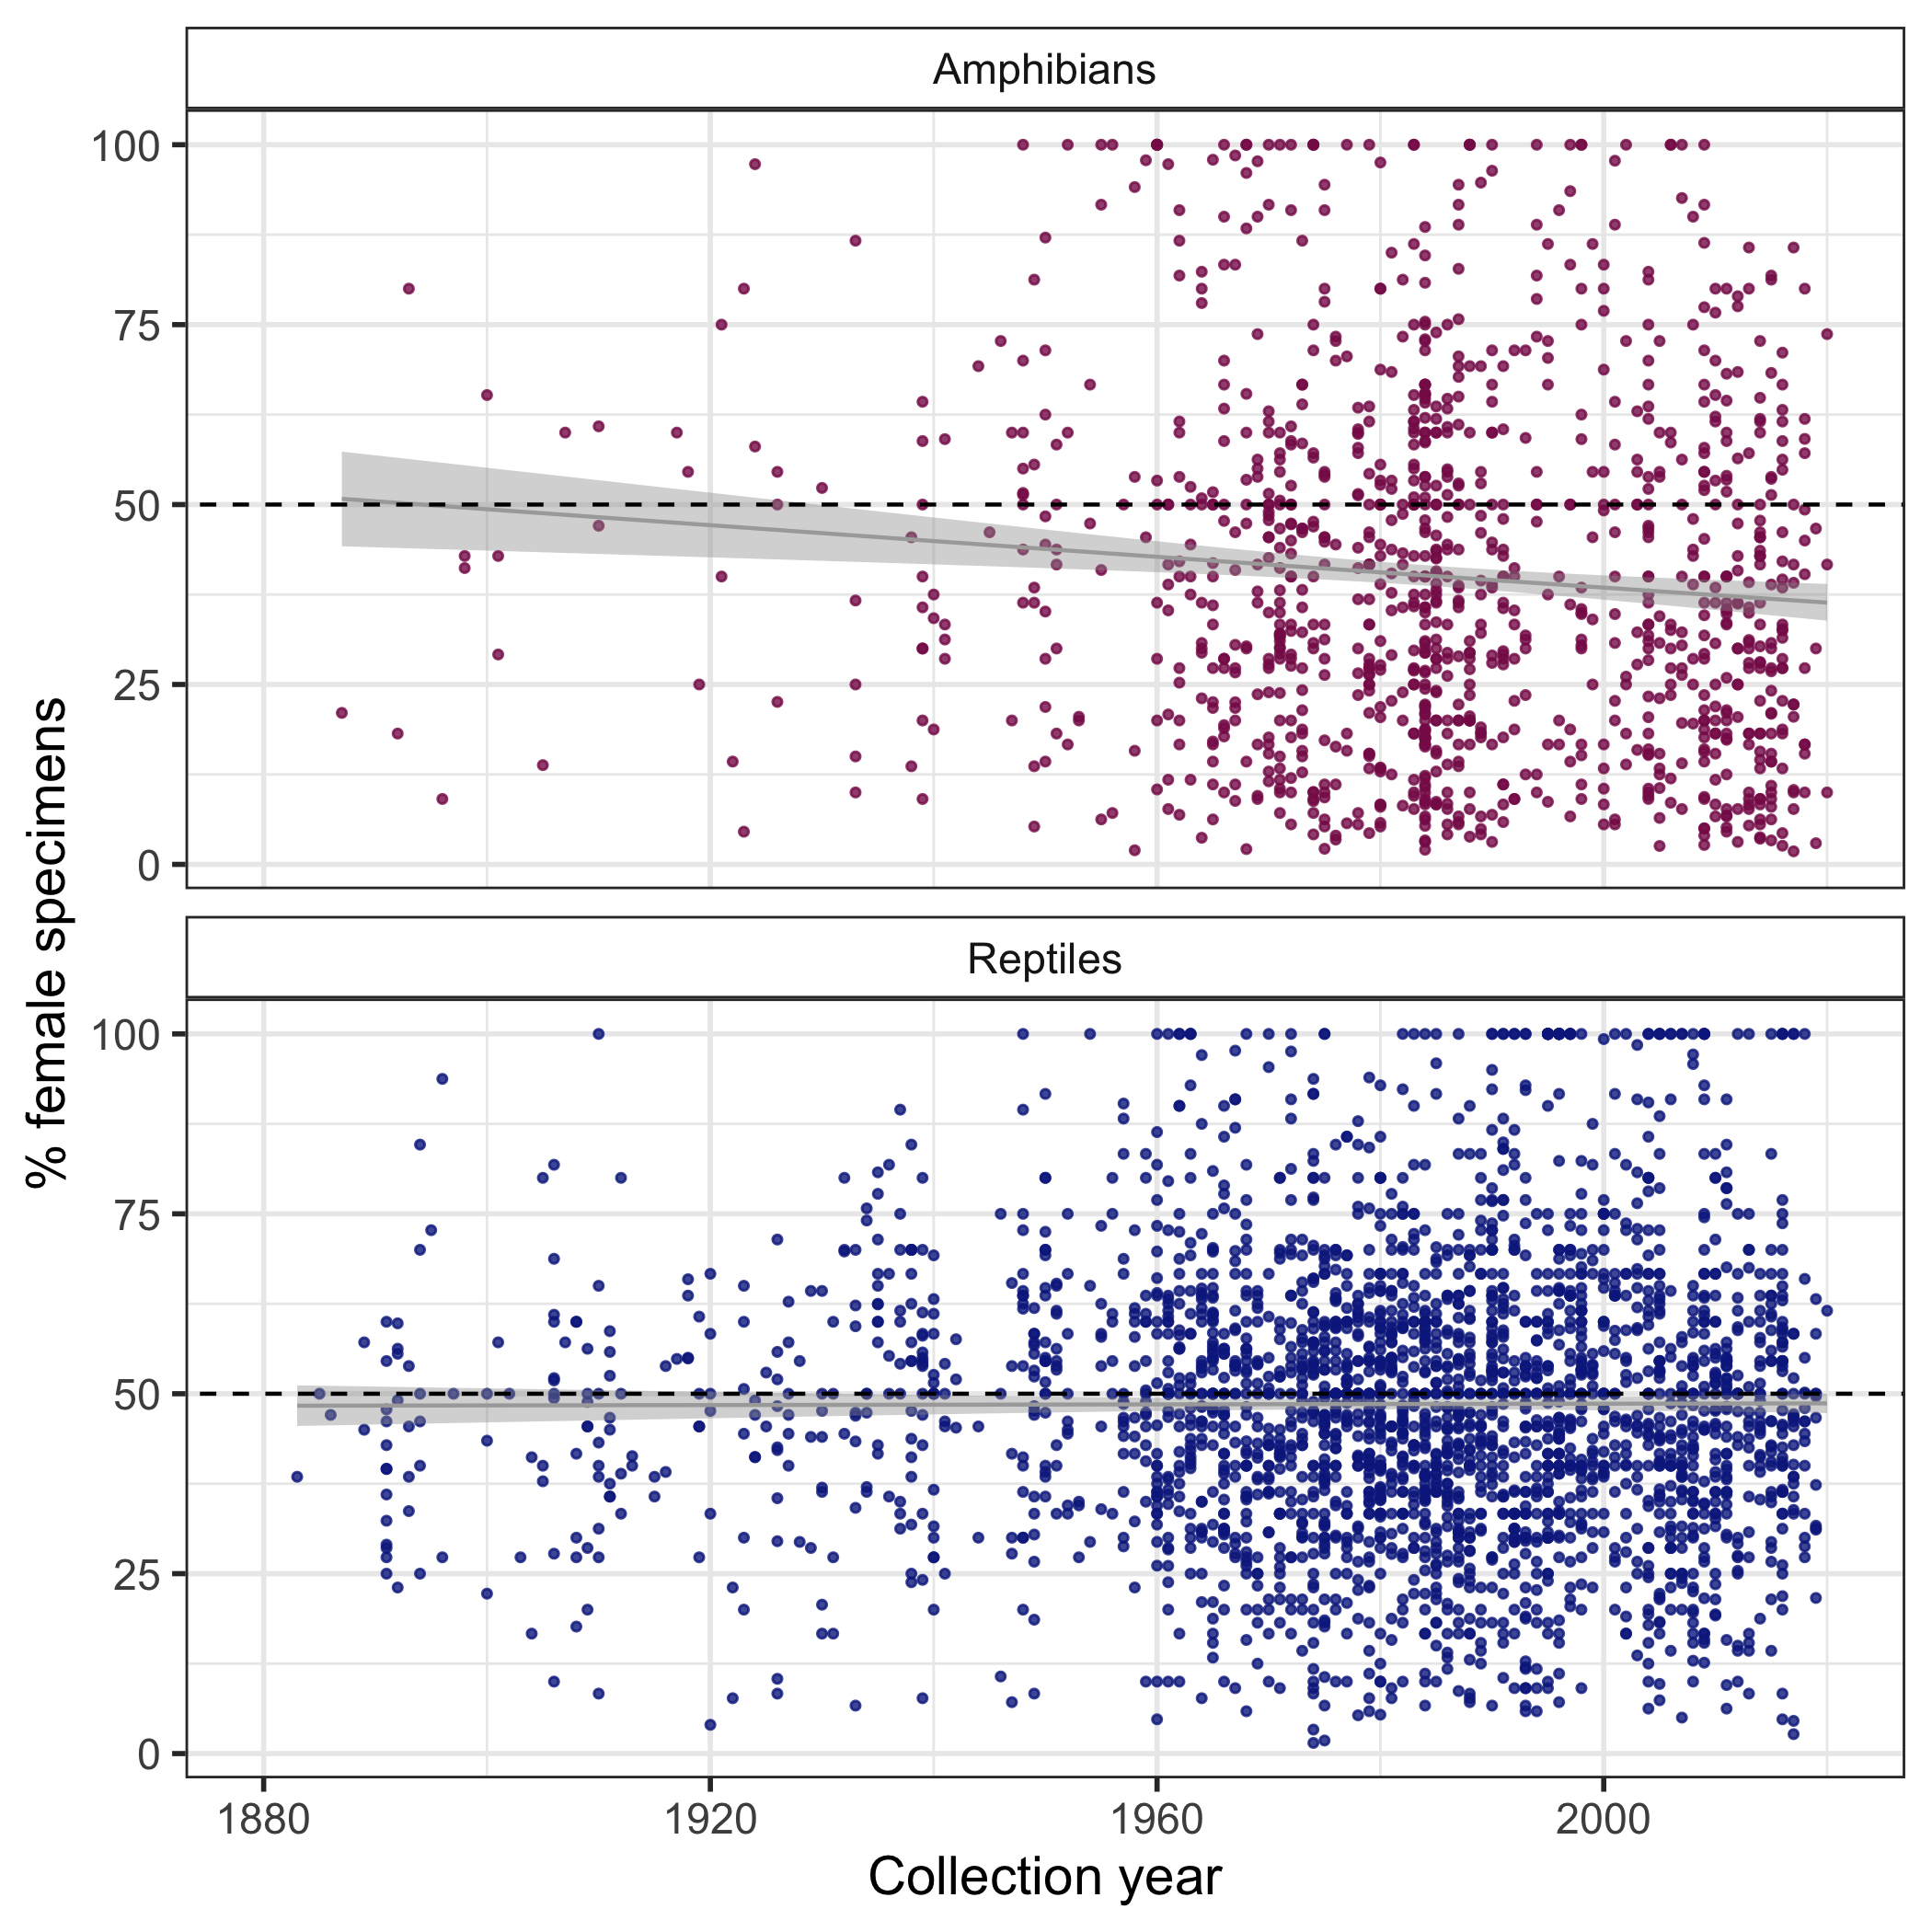
\includegraphics[scale = 0.4]{figures/years-all.png}
  \caption{Changes in the proportion of female specimens for each species collected each year between 1880 and 2010. 
  Best fit lines and 95\% confidence intervals from quasibinomial generalized linear models are shown in grey. 
  Data points represent species with at least 50 specimens collected in a given year. 
  The dashed line represents 50\% female specimens.
}
  \label{fig-time}
\end{figure} 

%-------------------------------------------------------------------------------
\newpage
\section{Male body mass and sexual size dimorphism.}

% figure A14
\begin{figure}[H]
 \centering
  \includegraphics[width = \linewidth]{figures/male-mass-all.png}
  \caption{Relationship between the percentage of female specimens for each species and log male body mass (g) for the species. 
  Only species with at least 100 specimens are included. 
  The dashed line represents 50\% female specimens. 
  Note that the x-axis scales are different for birds and mammals.
}
  \label{fig-male-mass}
\end{figure}

% figure A15
\begin{figure}[H]
 \centering
  \includegraphics[width = \linewidth]{figures/mass-orders-birds.png}
  \caption{Plots showing how \% female specimens in each species varies with male body mass (g) across the six largest orders of birds (from left to right, top to bottom: Passeriformes, Apodiformes, Piciformes, Psittaciformes, Charadriiformes, and Columbiformes). 
  Only species with at least 100 specimens are included. 
  The dashed line represents 50\% female specimens; grey lines show relationship between the variables using a simple linear regression and are for reference only. 
  Silhouettes are from PhyloPic.org contributed by Ferran Sayol (parrot, hummingbird, tit), Steven Traver (woodpecker) and Alexandre Vong (shorebird).}
  \label{fig-bird-male-mass}
\end{figure}

% figure A16
\begin{figure}[H]
 \centering
  \includegraphics[width = \linewidth]{figures/mass-orders-mammals.png}
  \caption{Plots showing how \% female specimens in each species varies with male body mass (g) across the six largest orders of mammals (from left to right, top to bottom: Rodentia, Chiroptera, Soricomorpha, Carnivora, Primates, and Artiodactyla). 
  Only species with at least 100 specimens are included. 
  The dashed line represents 50\% female specimens; grey lines show relationship between the variables using a simple linear regression and are for reference only. 
  Silhouettes are from PhyloPic.org contributed by Daniel Jaron (mouse), Yan Wong (bat), Becky Barnes (shrew), Lukasiniho (tiger), Sarah Werning (monkey), and Oscar Sanisidro (deer).}
  \label{fig-mammal-male-mass}
\end{figure}

% figure A17
\begin{figure}[H]
 \centering
  \includegraphics[width = \linewidth]{figures/ssd-orders-birds.png}
  \caption{Plots showing how \% female specimens in each species varies with sexual size dimorphism across the six largest orders of birds (from left to right, top to bottom: Passeriformes, Apodiformes, Piciformes, Psittaciformes, Charadriiformes, and Columbiformes).
  Sexual size dimorphism is male mass divided by female mass. 
  Only species with at least 100 specimens are included. 
  The dashed line represents 50\% female specimens; the dotted line is the point at which males and females have the same body size; grey lines show relationship between the variables using a simple linear regression and are for reference only. 
  Silhouettes are from PhyloPic.org contributed by Ferran Sayol (parrot, hummingbird, tit), Steven Traver (woodpecker) and Alexandre Vong (shorebird).}
  \label{fig-bird-ssd}
\end{figure}

% figure A18
\begin{figure}[H]
 \centering
  \includegraphics[width = \linewidth]{figures/ssd-orders-mammals.png}
  \caption{Plots showing how \% female specimens in each species varies with sexual size dimorphism across the six largest orders of mammals (from left to right, top to bottom: Rodentia, Chiroptera, Soricomorpha, Carnivora, Primates, and Artiodactyla). 
  Sexual size dimorphism is male mass divided by female mass. 
  Only species with at least 100 specimens are included. 
  The dashed line represents 50\% female specimens; the dotted line is the point at which males and females have the same body size; grey lines show relationship between the variables using a simple linear regression and are for reference only. 
  Silhouettes are from PhyloPic.org contributed by Daniel Jaron (mouse), Yan Wong (bat), Becky Barnes (shrew), Lukasiniho (tiger), Sarah Werning (monkey), and Oscar Sanisidro (deer).}
  \label{fig-mammal-ssd}
\end{figure}

%-------------------------------------------------------------------------------
\newpage
% SSD/mass model outputs
% Table A3
\input{figures/table-outputs}


%-------------------------------------------------------------------------------
\newpage
\section{Reverse sexual dimorphism in birds}

Some bird species show reverse sexual dimorphism, where females are larger or showier than the males. 
This occurs in hawks and vultures (Accipitridae), falcons (Falconidae), sandpipers and snipe (Scolopacidae), phalaropes (Charadriidae), jacanas (Jacanidae), skuas (Stercorariidae), boobies (Sulidae), frigate birds (Fregatidae), owls (Strigiformes), cuckoos (Cuculidae), hummingbirds (Trochilidae), manakins (Pipridae), and some ratites (Struthioniformes) (Swaddle et al. 2000\cite{swaddle2000novel}). 
The sexual size dimorphism and sexual plumage dimorphism analyses in the main text deal with this quantitatively and within the same framework as more typical male based sexual dimorphism. 
This is a better technique than lumping species into male versus female dominated dimorphism groupings, as the variation among sexes can vary hugely within these. 
For example, in European grouse species where the male capercaillie (\textit{Tetrao urogallus}) are more than twice the mass of females, while hazel grouse (\textit{Tetrastes bonasia}) females are only a gram heavier than males (Amadon, 1959\cite{amadon59}). 
However, our method had limitations - we did not have male and female body size for all species, and we only had plumage data for Passeriformes. 
As such we may have missed important patterns.

To deal with this, we divided the bird data into species where the female is generally the larger or showier sex (the families  Accipitridae, Falconidae, Scolopacidae, Charadriidae, Jacanidae, Stercorariidae, Sulidae, Fregatidae, Cuculidae, Trochilidae, Pipridae, and the orders Strigiformes and Struthioniformes), and species where the male is generally the larger or showier sex (all other species). We then compared the median percentage of females within species of the two groups, and fitted generalized linear models with quasibinomial errors to test for significant differences. 

Overall we found that the median percentage of females for species where the male was the larger or showier sex was 40\%, the same as for the whole dataset. 
For species where the female is the larger or showier sex the median percentage of females was 44.6\%, closer to the expected 50:50 ratio. 
There were significantly more females in species where the female is the larger or showier sex (quasibinomial GLM: $F_{1,1744} = 167.9$, $p < 0.001$; Figure \ref{fig-reverse})

% figure A19
\begin{figure}[H]
 \centering
  \includegraphics[width = \linewidth]{figures/female-extreme.png}
  \caption{Kernel density plots showing the \% female specimens in each species of bird for species where females are the larger or more showy sex (female extreme), or where males are the larger or more showy sex (male extreme). 
  Only species with at least 100 specimens are included. 
  The dashed line represents 50\% female specimens. }
  \label{fig-reverse}
\end{figure}

%-------------------------------------------------------------------------------
\newpage
\section{Ornamentation analyses in mammals}

\begin{table}[H]
\centering
\begin{tabular}{cccc}
 
  \hline
  \textbf{Model} & \textbf{Specimens} & \textbf{median \% female} & \textbf{Species}\\ 
  \hline
  Absent & 839,981 & 48.32 & 1,445\\
  Present & 17,403 & 39.52 & 67\\
  \hline
  \textbf{Feature} &&&\\
  \hline
  cheek extensions & 287 & 39.02 & 1\\
  horns or antlers & 13,506 & 38.86 & 50\\
  manes & 752 & 32.67 & 3\\
  nasal protrusions & 474 & 55.85 & 3\\
  ossicones & 157 & 49.68 & 1\\
  tusks & 2,227 & 48.05 & 9\\
  \hline
  \textbf{Order} &&&\\
  \hline
  Artiodactyla & 15,726 & 39.52 & 59\\
  Carnivora & 663 & 45.20 & 3\\
  Chiroptera & 188 & 55.85 & 1\\
  Primates & 826 & 35.85 & 4\\
  \hline

\label{table_orn_numbers}
\end{tabular}
\caption{Numbers of specimens and species with ornaments, divided by ornament type and order.} 
\end{table}

%-------------------------------------------------------------------------------
\newpage
% References
\bibliographystyle{vancouver}
\bibliography{sex-bias}

\end{document}